\chapter{Multi-scale modelling of dry granular flows}
\label{chapter:multiscale}

\ifpdf
    \graphicspath{{Chapter4/figs/raster/}{Chapter4/figs/pdf/}{Chapter4/figs/}}
\else
    \graphicspath{{Chapter4/figs/vector/}{Chapter4/figs/}}
\fi

\section{Introduction}

In nature, instabilities of slopes or cliffs can manifest themselves in 
dramatic events involving the sudden release of a large mass of soil. The 
prediction of these catastrophic 
events presents several challenges, one difficulty being our incomplete 
understanding of granular flow dynamics~\citep{Rondon2011}. Understanding 
the mechanics is of particular importance for risk assessment. Small scale 
laboratory experiments are usually unable to properly capture the 
dynamics of geophysical events. However, they can be useful to precisely study 
the physical mechanisms, which may play a crucial role in real 
flows~\citep{Iverson1997}. 

Conventionally, granular materials such as soils are modelled as a continuum. 
On a macroscopic scale, granular materials exhibit many collective phenomena 
and the use of continuum mechanics to describe the macroscopic behaviour can be 
justified. However on a grain-scale, granular materials exhibit complex 
solid-like and/or fluid-like behaviour depending on how the grains interact 
with each other. Numerical studies at grain-scale allow a precise 
understanding of the internal flow structure. However, even in simplified 
geometries such as those investigated in the laboratory-scale experiments, DEM 
suffers from a serious short-coming in the number of grains that can be 
simulated in a reasonable time. This is a critical issue for more complex 
geometries or when granular processes which occur on a long time-scale are 
considered. For this reason, most numerical studies are 
performed in 2D or simple particles shapes and size distributions are 
considered. 

Classical modelling strategies based on the finite element method (FEM) cannot 
be used for the simulation of very large deformations due to mesh distortion 
effects. In various applications of FEM, this problem is treated by means of 
technical 
tools such as re-meshing. These methods are, however, not robust and lead to 
round-off errors and are sensitive to the mesh characteristics. Recent works on 
granular materials suggest that a continuum law may be incapable of revealing 
in-homogeneities at 
the grain-scale level, such as orientation of force chains, collapse of local 
voids and grain rearrangements, which are purely micro-structural 
effects~\citep{Rycroft2009a}. Discrete element approaches 
are capable of simulating granular materials as discontinuous systems
allowing one to probe into local variables such as position, velocities, 
contact forces, etc. The fundamental question is how to model granular 
materials which exhibit complex phenomena. It is important to understand the 
mechanics of granular flows and the ability and limitations of continuum 
methods in modelling the granular flow dynamics. 

\section{Granular column collapse}
\label{sec:dry_granular_column}
The collapse of a granular column, which mimics the collapse of a cliff, has 
been extensively studied in the case of dry granular 
material~\citep{Lube2005,Lajeunesse2004,Kerswell2005,Zenit2005,Staron2007a,Hogg2007,Lo2009}.
The granular column collapse experiment involves filling a rectangular channel 
of height $H_0$ and width $L_0$ with a granular material of mass 
\textit{m} (\cref{fig:exp}). The granular column is then released \textit{en 
masse} by quickly removing the gate, thus allowing the granular material to 
collapse onto a horizontal surface, forming a deposit having a final height 
$H_f$ and length $L_f$. Despite the complexity of the intermediate flow 
dynamics, experimental investigations have shown that the flow evolution, the 
spreading velocity, the final extent of the deposit, and the energy dissipation 
can be scaled in a quantitative way independent of the substrate properties, 
grain size, density, the shape of the granular material and the released 
mass~\citep{Staron2007a,Lajeunesse2005,Lube2005}. Granular collapse has 
also been studied using DEM, which allows precise measurement of the internal 
flow structure~\citep{Lo2009,Staron2005,Staron2007a,Utili2014}. Power laws 
relating the final run-out and height to the initial aspect ratio ($a = H_0 / 
L_0$) of the column were observed. These findings immediately pose a question: 
are these simple scaling laws fortuitous, an oversimplification, or in fact 
indicative of a simple dynamical balance? 


Granular flows are conventionally modelled as a frictional dissipation process 
in continuum mechanics but the lack of influence of inter-particle friction on 
the energy dissipation and spreading dynamics~\citep{Lube2005} is surprising. 
However,~\citet{Kerswell2005} showed the run-out behaviour has a clear material 
dependence. Although, the collapse of a granular column on a horizontal surface 
is a simple case of granular flow, a proper model that describes the flow 
dynamics is still lacking. Simple mathematical models based on conservation of 
horizontal momentum capture the scaling laws of the final deposit, but fail to 
describe the initial transition regime. From a theoretical point of view, the 
spreading has been described using depth averaged 
equations~\citep{Kerswell2005,Larrieu2006}. The depth-averaged and 
Saint-Venant equations, however, struggle to recover the precise dynamic 
behaviour of the system~\citep{Warnett2013} and only succeed in predicting the 
scaling observed for an aspect ratio less than one. Describing the behaviour of 
cases with larger aspect ratios and capturing the initial stage of the 
collapse, when the grains experience a rapid change of direction from vertical 
to horizontal, remain open challenges.


In the present study, multi-scale numerical modelling, i.e. grain-scale 
modelling and continuum analyses, of the quasi-two-dimensional collapse of 
granular columns are performed using two-dimensional the Discrete Element 
Method (DEM) and the Generalised Interpolation Material Point Method (GIMP 
method). The GIMP method, a hybrid Eulerian--Lagrangian approach, with a 
Mohr-Coloumb failure criterion is used to describe the continuum behaviour of 
the granular column collapse. Whereas, the micro-mechanics of the flow is 
captured using DEM simulations. In this section, the run-out behaviour of 
quasi-two-dimensional collapse using both MPM and DEM will be studied for 
initial aspect ratios varying from 0.2 to 
10. The flow kinematics and the run-out behaviour between the grain-scale and 
the continuum simulations highlights the limitations of the continuum approach 
in modelling dense granular flows and their ability in capturing the complex 
flow kinematics which are due to micro-scale rheology.

\subsection{Numerical set-up}

In this study, the numerical set-up of granular column collapse is analogous to 
the  experimental investigation performed by~\citet{Lajeunesse2004}. The 
experimental configuration of~\citet{Lajeunesse2004} is shown in 
\cref{fig:exp}. A granular material of mass \textit{m} was poured into a 
container to form a rectangular heap of length ${L}_{0}$ and height 
${H}_{0}$. The internal friction angle and the wall friction between the wall 
and the glass beads measured by~\citet{Lajeunesse2004} are listed 
in~\cref{table:mat_prop}. The gate was then quickly removed to release the 
granular mass that spreads in the horizontal channel until it comes to rest. 
The final run-out distance ${L}_{{f}}$ and the collapsed height $H_{{f}}$ were 
measured. The run-out distance and collapse height exhibit a power law relation 
with the initial aspect ratio `\textit{a}' $(=H_{0}/L_{0})$ of the column. 

\begin{table}[tbhp]
\caption{Material properties of glass ballotini used in granular column 
collapse~\citep{Lajeunesse2004}.}
\label{table:mat_prop}
\centering
\begin{tabular}{ll}
\toprule
\textbf{Parameter} & \textbf{Value} \\ \midrule
Mean grain diameter & 1.15~\si{\mm} \\
Repose angle & 22$\pm 0.5$\si{\degree} \\
Avalanche angle & 27.4$\pm 0.5$\si{\degree} \\
Wall friction angle & 24.8$\pm 0.2$\si{\degree}\\
\bottomrule
\end{tabular}
\end{table}


Granular materials when released suddenly on a 
horizontal surface exhibit transient flow. In this study, the mechanism of flow 
initiation, spreading dynamics and energy dissipation are studied for varying 
initial aspect ratios of the granular column. The particle size distribution 
(PSD) is one of the most important factors controlling landslide initiation and 
soil permeability~\citep{Utili2014}. Due to the non-availability of the PSD 
used in the experiment, a PSD curve was generated that matches the range of 
grain size used in the experiment. A cumulative $\beta$ distribution 
(described in~\cref{sec:beta_dist}) was used to generate a graded sample with a 
mean grain diameter of 1.15\si{\mm} (\cref{fig:PSD}). 
The DEM sample was composed of $\sim3000$ disks with a uniform distribution of 
diameters by volume fractions in the range $[d_{min}, d_{max}] = 0.92 - 1.38$ 
\si{\mm} with poly-dispersity $r = \frac{d_{max} }{d_{min}} = 1.5$. The number 
of DEM grains used in this study is relatively small due to the practicality of 
simulating coupled fluid-grain interactions at a large scale. Coupled 
fluid-grain simulations are computationally very expensive. Nevertheless, this 
study utilises sophisticated hardware and software technologies, available at 
this time, to simulate the largest possible REVs that provide reasonable 
description of granular flow behaviour.~\citet{Marketos2009} observed that the 
boundary-grain interface may influence the fabric and voids ratio of the 
material in contact. The boundary effect is found to extend up to 2 mean grain 
diameters from a smooth, solid boundary over which the granular material had 
been placed. Sufficient number of grains are used to avoid any such boundary 
effects. 

The granular column was prepared by allowing randomly placed grains to undergo 
ballistic deposition with a constant potential head between layers of soil 
grains. A snapshot of the sample generated is shown in~\cref{fig:a4b4r18}. A 
DEM sample with soil grains arranged in a regular hexagonal lattice was also 
used to understand the influence of crystallisation and jamming on the run-out 
behaviour. 

\begin{figure}[tbhp]
\centering
\begin{subfigure}[b]{0.95\textwidth}
\centering
\includegraphics[width=0.4\textwidth]{a4b4r18}
\caption{A snapshot of a DEM sample prepared using ballistic deposition 
technique.}
\label{fig:a4b4r18}
\end{subfigure}
\\
\begin{subfigure}[b]{0.75\textwidth}
\centering
\includegraphics[width=\textwidth]{PSD}
\caption{Particle size distribution of the DEM sample generated using the 
cumulative $\beta$ distribution approach.}
\label{fig:PSD}
\end{subfigure}
\caption{The DEM sample used for the granular column collapse simulation and 
its grain size distribution curve.}
\label{fig:DEM_Sample}
\end{figure}


The overlap between grains is determined by the stiffness 
$\textit{k}_{{n}}$ of the spring in the normal direction. Typically, 
an average overlap in the range 0.1 to 1.0\% is desirable~\citep{Zenit2005} and 
the spring constant is chosen to produce grain overlaps in this range. The 
stiffness is determined as
\begin{align}
& \textit{k}_{{n}}=\frac{2 \pi 
G}{(1-\nu)\left[2\ln(\frac{2r}{A})-1\right]} \\ 
& A = \left[\frac{2r(1-\nu)f_{n}}{\pi G}\right]^{\frac{1	}{2}}\,,
\end{align}
where $f_{n}$ is the normal contact force; G is the shear modulus; $\nu$ is the 
Poisson's ratio and r is the radius of the grain. A simpler form of stiffness 
for a spherical grain is defined as
\begin{equation}
\textit{k}_{{n}}=4Er\,,
\end{equation}
\nomenclature[a-E]{\textit{E}}{Young's modulus of the material}
where \textit{E} is the Young's modulus of the material and \textit{r} is the 
radius of the grain.~\citet{Cambou2009} observed that the contact model has 
negligible influence on the run-out behaviour of rapid granular flows. The 
granular collapse simulations performed using non-linear Hertz-Mindlin contact 
model and the linear-elastic contact model showed no significant difference in 
the granular flow behaviour~\citep{Utili2014}. A linear-elastic contact model 
is used in the present study due to its simplicity and lower computation time 
requirement. The maximum tangential force is limited by the Mohr-Coloumb 
criterion. 

\citet{Staron2007a} observed that the coefficient of restitution $\varepsilon$ 
dramatically changes the behaviour of the system as $\varepsilon\rightarrow 
1$; in particular, this dramatic change is expected to become more important 
for increasing values of \textit{a}. On the contrary, for $\varepsilon \le 
0.8$, the influence of the coefficient of restitution becomes negligible. In 
the present study, a value of 0.75 is adopted as the coefficient of 
restitution, similar values were adopted 
by~\citet{Girolami} and~\citet{Zenit2005}. The normal damping coefficient 
$C_{{n}}$ is appropriately chosen to achieve the required coefficient of 
restitution 
$\varepsilon$:
\begin{align}
& C_{{n}}=2\gamma \sqrt{m_{{ij}}k_{{n}}} \,,\\ 
& \mbox{where} \quad \gamma = -\frac{\ln(\varepsilon)}{\sqrt{\pi^{2}+\ln^2 
(\varepsilon)}},\quad \mbox{and} \quad 
\textit{m}_{{ij}}=\frac{\textit{m}_{{i}}\textit{m}_{{j}}}{\textit{m}_{{i}}
 + \textit{m}_{{j}}} \,.
\end{align}
%
The micro-mechanical parameters used in this study are presented 
in~\cref{table:DEM_data}. A rolling resistance was adopted in order to 
model the shape effect of non-spherical grains~\citep{Iwashita1998}. Due to the 
unsteady nature of the flow, the grains get dispersed on the horizontal plane 
as discrete bodies start to separate from the main mass, hence the run-out 
distance is calculated as the position of the farthest grain which has at least 
one contact with the main mass.
%

The configuration of the granular column collapse using DEM is show 
in~\cref{fig:DEM_Column_Sample} for a column with an initial aspect ratio of 
0.8. The soil grains were packed using ballistic deposition technique once a 
stable state was reached, the gate was opened allowing the granular column to 
collapse and flow. Frictional boundaries were specified on the left and 
the bottom boundaries.

\begin{figure}
\centering
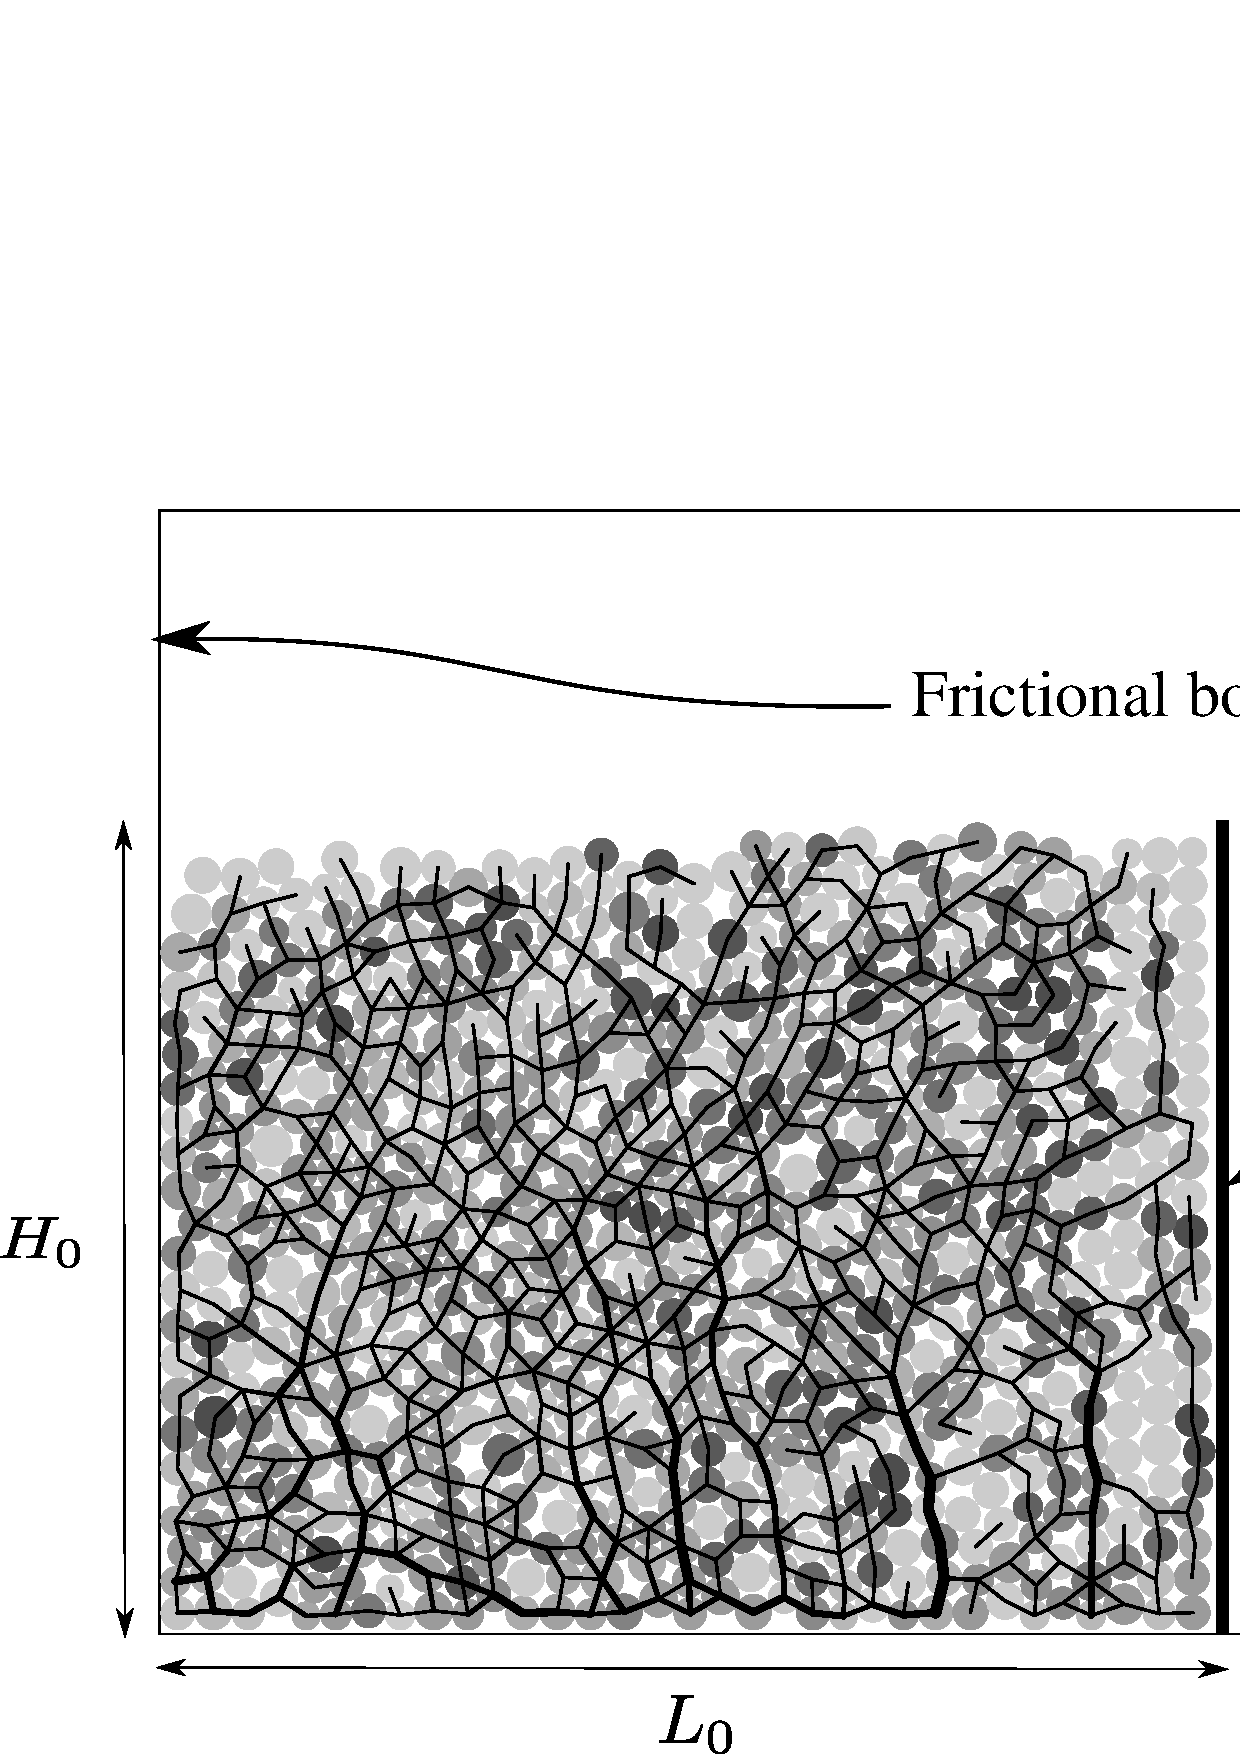
\includegraphics[width=0.95\textwidth]{DEM_Column_Sample}
\caption[DEM set-up of a granular collapse simulation (\textit{a} = 0.8).]{DEM 
set-up for a granular collapse simulation (\textit{a} = 0.8). 
Shows the grains in a stable state under the influence of gravity.}
\label{fig:DEM_Column_Sample}
\end{figure}

\begin{table}
\caption{Micro-mechanical parameters used in DEM simulations of granular column 
collapse.}
\label{table:DEM_data}
\centering
\begin{tabular}{ll}
\toprule
\textbf{Parameter} & \textbf{Value} \\ \midrule
Young's modulus of glass bead & 
$70\times10^{9}$~\si{\newton\per\m\squared}\\ 
Poisson's ratio & 0.22 - 0.24\\ 
Diameter of glass beads & 0.92 to 1.38~\si{\mm}\\
Normal and shear stiffness of grains & $1.6 \times 
10^{8}$~\si{\newton\per\m}\\ 
Normal and sear stiffness of wall & $4 \times 
10^{8}$~\si{\newton\per\m}\\
Inter-particle friction coefficient, $\mu$ & 0.53 \\
Wall friction coefficient & 0.466 \\ 
Coefficient of restitution, $\varepsilon$ & 0.75 \\ 
Rolling spring constant  & $1.0\times10^3$~\si{\newton\meter\per\radian}\\ 
Coefficient of rolling damping & $1.0 \times 
10^{-1}$~\si{\newton\meter\second\per\radian} \\ \bottomrule
\end{tabular}
\end{table}
\nomenclature[g-nu]{$\nu$}{Poisson's ratio (or) Fluid viscosity}
\nomenclature[g-Phi]{$\Phi$}{Dilatancy angle}
\nomenclature[a-Dr]{$D_r$}{Relative density}
\nomenclature[s-y]{\textit{y}}{Yield or failure}
The GIMP method with a Mohr-Coloumb constitutive model was used to simulate 
plane strain collapse of granular columns.~\citet{Crosta2009a} observed that 
the Mohr-Coloumb model with non-associate flow rule is able to capture granular 
collapse dynamics and models the strong vertical motion. This method does not 
suffer the limitations of typical shallow water equation techniques. In order 
to understand the ability and limitations of continuum approaches in capturing 
the local rheology, it is important to scale the grain-scale material 
properties, such as the inter-particle friction and stiffness, to the continuum 
scale (macroscopic friction and Young's modulus).~\citet{Crosta2009a} observed 
that the friction angle plays a significant role on the run-out behaviour. 

In the MPM simulations, the granular flow was assumed to be in the critical 
state and the critical state friction angle was used as an input in the 
Mohr-Coloumb model. In order to obtain the critical state friction angle of the 
granular sample, a shear test is performed using 1078 DEM grains. A 
bi-periodic boundary condition was adopted on the sides of the sample 
(\cref{fig:shear}). Two layers of fixed grains (shown in black) were placed at 
the top and the bottom of the shear sample. A normal stress $\sigma_n^\prime$ 
and a horizontal velocity \textit{v} was applied to the fixed grains at the top 
of the shear sample. As the normal effective stress was varied, the average 
shear stress in the sample was measured. The stresses were smoothed by 
averaging across time steps. The sample was sheared until the critical state 
was reached. The slope of shear stress versus normal effective stress gives the 
critical state friction angle. A critical state friction angle of 
$22.2$\si{\degree} was obtained. The macroscopic friction angle was in the 
range observed by~\citet{Estrada2008} and~\citet{Mitchell2005}. The Young's 
modulus of the granular assembly was obtained as the initial slope of the 
stress-strain plot of a uni-axial compression of a laterally confined granular 
column using DEM.

\begin{figure}
\centering
\begin{subfigure}[b]{0.5\textwidth}
\centering
\includegraphics[width=\textwidth]{simple_shear}
\caption{Boundary conditions}
\label{fig:shear}
\end{subfigure}\\
\begin{subfigure}[b]{0.65\textwidth}
\centering
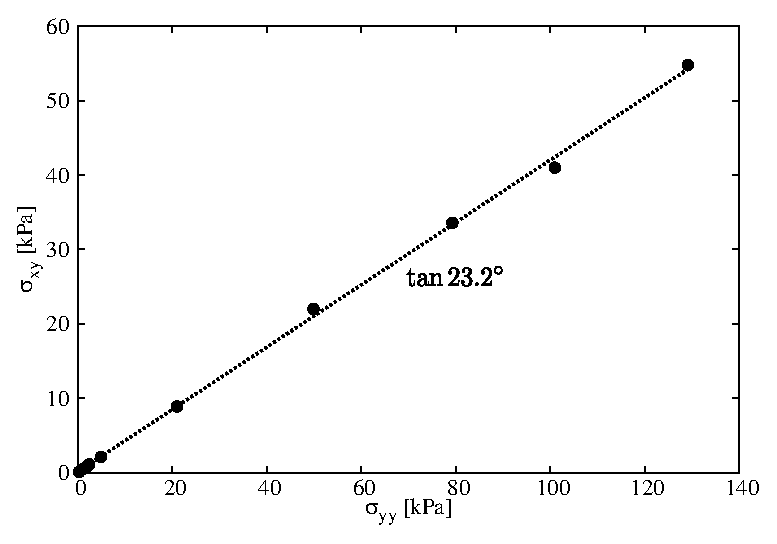
\includegraphics[width=\textwidth]{Sxy_vs_Syy}
\caption{Critical state friction angle from periodic shear test}
\label{fig:Sxy_vs_Syy}
\end{subfigure} 
\caption{Periodic shear test using DEM to obtain macroscopic friction angle.}
\label{fig:shear_test}
\end{figure}

\citet{Guilkey2003} suggests using at least four material points per cell for 
large deformation problems. In the present study there were 16 material points 
per cell. If the mesh is too fine and the number of particles is too 
large, the particle size $2lp$ decreases, and the GIMP interpolation 
function tends to approach the original MPM function, as shown 
by~\citet{Bardenhagen2004}. Hence, GIMP loses the merit that it reduces the 
numerical noise due to material points crossing the background mesh. In 
addition, the probability of particles crossing the background mesh increases 
with decrease in the mesh size, hence, more noise may be 
produced~\citep{Abe2013}. The effect of the number of material points per cell 
on the run-out behaviour is discussed later in~\cref{sec:MPM_points_per_cell}.

The initial set-up of a granular column collapse (a = 1) using MPM is shown 
in~\cref{fig:MPM_Sample}. For all the MPM simulations, a cell size of 
$2\times10^{-3}\si{\m}$ with 16 material points per cell was adopted 
(\cref{fig:ini_mesh_mpm_column}). The granular columns were
discretised into 40,000 to 160,000 material points. Each material point 
represents one-eigth of a DEM soil grain. Since, the scale of the problem being 
modelled is small and it is important to precisely define the flow surface, a 
larger number of material points are used to represent the geometry. The 
initial vertical effective stress simulated in MPM, before the collapse stage, 
is shown in~\cref{fig:ini_stress_mpm_column}. The extent of the 
background mesh in MPM is much larger than the initial column. In MPM, the 
material points move inside the grid, so it is important to have a sufficiently 
large domain for the collapse. Frictional boundaries are applied as constrains 
on the nodal accelerations on the left and the bottom boundaries. The 
parameters used for the continuum analyses are presented 
in~\cref{table:MPMData}. 

\begin{table}
\caption{Parameters used in continuum simulations of granular column collapse.}
\label{table:MPMData}
\centering
\begin{tabular}{ll}
\toprule
\textbf{Parameter} & \textbf{Value} \\ \midrule
Material point spacing & 0.5~\si{\mm} \\
Number of material points per cell & 16 \\
Mesh length & $2\times10^{-3}\si{\m}$  \\
Young's Modulus, E & $1.98 \times 10 ^{6}$~\si{\N\per\m\squared} \\
Poisson's ratio, $\nu$ & 0.22 to 0.24 \\ 
Friction angle, $\phi$ & $22.2 \pm 0.2\si{\degree}$ \\
Dilatancy angle, $\varPhi$ & $0$\si{\degree} \\
Density, $\rho$ & 1925~\si{\kg\per\m\cubed}\\
Wall friction & 0.466 \\
Time step increment & $1.0 \times 10^{-6}$~\si{\second}\\ \bottomrule
\end{tabular}
\end{table}

\begin{figure}[tbhp]
\centering
\begin{subfigure}[b]{0.95\textwidth}
\centering
\includegraphics[width=0.95\textwidth]{ini_mesh_mpm_column}
\caption{Initial arrangement of material points in the mesh. Closer view of 
16 material points per cell for a column with an initial aspect ratio of 1. 
Cell size of $2\times10^{-3}\si{\m}$.}
\label{fig:ini_mesh_mpm_column}
\end{subfigure}
\\
\begin{subfigure}[b]{0.95\textwidth}
\centering
\includegraphics[width=0.95\textwidth]{ini_stress_mpm_column}
\caption{Initial vertical effective stress in MPM for a column with an aspect 
ratio of 1.}
\label{fig:ini_stress_mpm_column}
\end{subfigure}
\caption{MPM initial mesh and vertical stress for a granular column collapse 
simulation (\textit{a}=1).}
\label{fig:MPM_Sample}
\end{figure}



\subsection{Deposit morphology}
A series of two-dimensional plane-strain MPM and DEM simulations of granular 
column collapse were performed by varying the initial aspect ratio of the 
column from 0.2 to 10. The evolution of run-out and the flow kinematics 
observed in both approaches were compared to understand the ability and 
limitations of these approaches. The normalised final run-out distance, $\Delta 
L = (L_{{f}}-L_{0})/L_{0}$, as a function of the initial aspect ratio 
\textit{a} of the column is presented in~\cref{fig:run-out}. Similar to the 
experimental behaviour a power law relation between the run-out 
and the initial aspect ratio of the column is observed. Two distinct flow 
regimes can be seen: (a) for \textit{a} < 2.7 a linear relation between the 
spread and aspect ratio can be observed, and (b) for \textit{a} > 2.7 a 
power-law relationship exists. In the present study, the following scaling law 
for the run-out (using DEM) is observed:
%
\begin{equation}
\frac{L_{{f}}-L_{0}}{L_{0}} \approx  
\begin{cases}
1.67 a, &\qquad \textit{a}\lesssim 2.7 \\
2.7 a^{2/3}, &\qquad \textit{a} \gtrsim 2.7 \\
\end{cases}
\end{equation}
Both, MPM and DEM simulations are able to capture the linear relationship for 
\textit{a} < 2.7, and the simulation results agree with the experimental 
investigation~\citep{Lajeunesse2005}. This shows that a simple frictional 
dissipation model is able to capture the flow dynamics for columns with small 
aspect ratios. For \textit{a} < 2.7, the normalised run-out distances predicted 
using DEM simulations are very close to those observed in the experiment. DEM 
simulations with a hexagonal packing show shorter run-out distances in 
comparison to the randomly packed sample. This difference in the run-out 
behaviour might be due to crystallisation and jamming effects in hexagonal 
packing. The small difference in the final run-out between the DEM and the 
experimental results can be attributed to the variation in the packing of 
grains and the three-dimensional grain shape. Also, the experimental data 
corresponds to granular column collapse in a rectangular channel, where the 
collapse is not the pure two-dimensional collapse that is in the case of 
numerical simulations. Most aerial and sub-marine landslides have a large 
lateral extent, i.e., plane-strain condition, hence in the present study 
two-dimensional simulations are performed. Although two-dimensional simulations 
don't capture movement of the grains perpendicular to the plane of the 
experiment, it simplifies the configuration so as to compare DEM simulations 
with MPM. Also,~\citet{Balmforth2005} observed that the side-walls 
in quasi-two-dimensional collapse do not influence the power-law behaviour 
but affect the numerical constant, which depends on the material properties. 

A significant difference in the final run-out between MPM, which is based on a 
simple frictional model for dissipation of potential energy, and DEM 
simulations, indicates a change in the mechanism of energy 
dissipation for columns with large aspect ratios (\textit{a} > 
2.7). A transition in the run-out behaviour at an aspect ratio of 2.7 indicates 
a change in the flow kinematics. Similar behaviour in the run-out distance was 
observed by~\citet{Bandara2013} for columns with large aspect ratios ($a \ge 
2$).~\citet{Mast2014} observed a 40\% increase in the final run-out distances, 
for large aspect ratios, than reported in the literature. Previous studies have 
failed to describe the mechanism of energy dissipation in continuum approaches 
and the reason for longer run-out distance.~\Cref{sec:energy} discusses the 
reason behind the difference in the run-out behaviour between continuum and 
experimental findings.

The longer run-out distance in MPM simulations at large aspect ratios might be 
influenced by the amount of material mobilised during the collapse. In tall 
columns, the entire column participates in the flow, in contrast to short 
columns where the collapse is due to avalanching of the flanks. It is possible 
that MPM simulations collapse more resulting in longer run-out 
distances.~\Cref{fig:height} shows the normalised final height as a function of 
the initial aspect ratio of the column. Similar to the run-out behaviour, the 
normalised-height also shows two distinct regimes. The scaling of final height 
of the column with the initial aspect ratio of the column can be written as
\begin{align}
\frac{H_{{f}}}{L_{{i}}} \propto  
\begin{cases}
\textit{a}, \qquad & \textit{a}\lesssim0.7 \\
\textit{a}^{2/3}, \qquad & \textit{a}\gtrsim0.7 \\
\end{cases}
\end{align} 

The final heights predicted by both DEM and MPM simulations match the 
experimental data for columns with smaller aspect ratios ($a \le 0.7$). A 
linear relationship between the final height and the aspect ratio indicates 
that only a part of the granular column is mobilised during the collapse. For 
tall columns, both approaches predict similar normalised heights. However, the 
normalised height observed in MPM is higher than in DEM simulations, which is 
in contrast to the idea of an increase in the amount of material mobilised 
during the collapse in MPM simulations resulting in longer run-out distance. 
Hence, the longer run-out observed in MPM simulations is due a change in the 
flow dynamics at higher aspect ratios, which is not captured in MPM 
simulations. The final height of a column is controlled by the amount of static 
region in the granular column collapse, while the run-out distance is 
essentially a function of the flowing mass. Hence, it is important to compare 
the evolution of flow and the internal flow structure in DEM and MPM 
simulations.

\begin{figure}[tbhp]
\centering
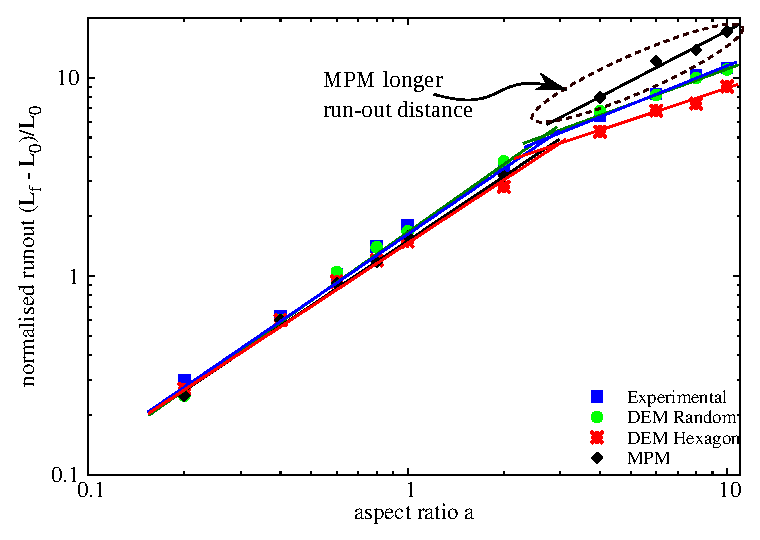
\includegraphics[width=\textwidth]{runout}
\caption{Normalised final run-out distance for columns with different initial 
aspect ratios.}
\label{fig:run-out}
\end{figure}

\begin{figure}[tbhp]
\centering
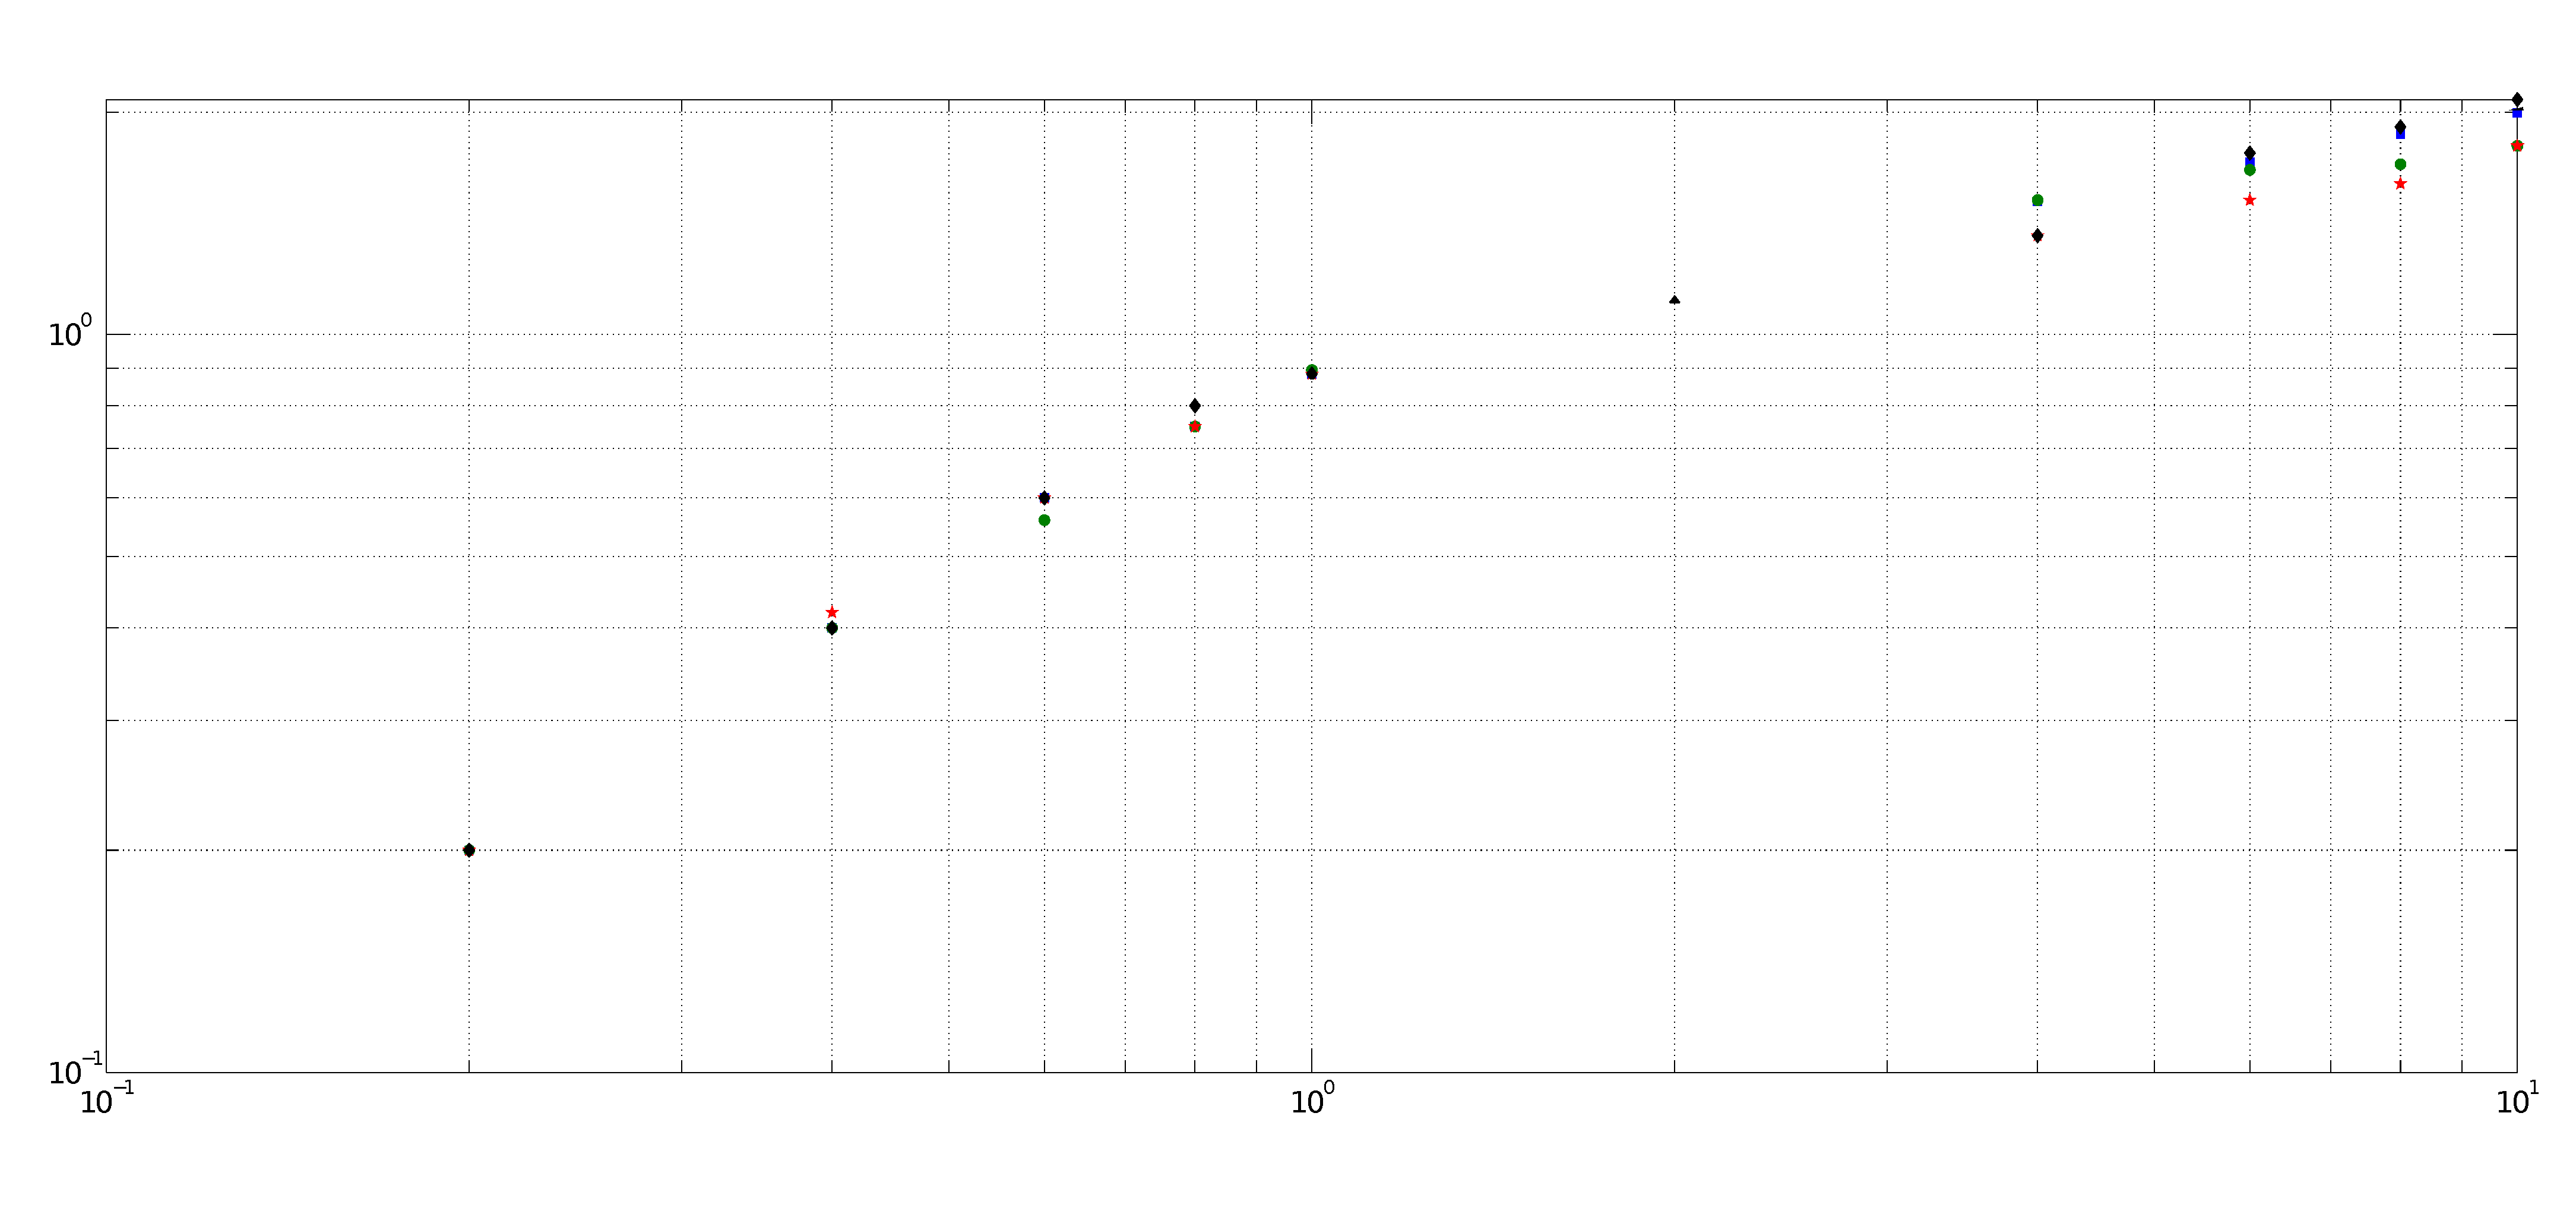
\includegraphics[width=0.975\textwidth]{height}
\caption{Normalised final collapse height for columns with different initial 
aspect ratios.}
\label{fig:height}
\end{figure}

\subsection{Flow evolution and internal flow structure}

The normalised run-out and height as a function of the aspect ratio indicate 
that, for a given granular material and substrate properties, the flow dynamics 
and the final deposit morphology are independent of the volume of granular 
material released, but depend only on the geometry of the column. A 
power law relationship is observed between the run-out distance and the initial 
aspect ratio of the column. A transition in the run-out behaviour at an aspect 
ratio of 2.7 indicates a change in the flow dynamics. 


Dimensional analysis of granular column collapse reveals an intrinsic time 
defined as $\sqrt{H_{0}/g}$. This intrinsic time is a transient time 
of order $\tau_{c}$, at which the flow is fully developed, i.e., the potential 
energy available at the initial stage of collapse is now fully converted to 
kinetic energy. Numerical simulation of the velocity profile of a granular 
column (\textit{a}=0.4) at the critical time $\tau_{c}$ is presented in 
\cref{fig:a04tc}. At the critical time, the velocity field depends only on the 
position of the grain along the sliding mass. The maximum velocity is observed 
at the front of the flowing mass corresponding to that of a plug flow in the 
horizontal direction. Particulate and continuum simulations show similar 
run-out distances at the critical time. Both approaches show similar quantities 
of material 
destabilised above the failure surface. However, the crystalline arrangement of 
soil grains in a hexagonal packing results in a different flow mechanics, which 
also shows the effect of jamming at the flow front. The continuum nature of MPM 
results in a slightly different geometry of the material destabilised above the 
failure surface in comparison to DEM simulations. The velocity profile is 
similar to a steady granular surface flow observed by~\citet{Lajeunesse2004}. 


For short columns (\textit{a} < 2.7), the flow is initiated 
by a failure at the edge of the pile along a well-defined shear-failure surface.
The granular mass fails through avalanching of flanks producing a 
truncated cone-like deposit (`\textit{a}' < 0.7) or conical deposit 
(`\textit{a}' > 0.7). The grains located above the failure surface move 
``\textit{en masse}'' leaving a static region underneath the failure surface. 
For columns with lower initial aspect ratios, the run-out distance is 
proportional to the mass flowing above the failure surface. The spreading 
results from a Coulomb-like failure of the edges and implies no free fall of 
the column. In this case, the effective friction 
properties of the flow can be simply predicted from the shape of the final 
deposit. The amount of mass mobilised during the collapse is significantly 
affected by the angle of the failure surface.

\Cref{fig:a04tc} shows that both 
numerical techniques predict a distinct failure surface when the flow is fully 
developed at critical time $\tau_{{c}}$. The angle of the failure 
surface is found to be about $55\si{\degree}$. The failure surface begins from 
the toe of the column and propagates inwards at an angle of $50$ to 
$55\si{\degree}$. The formation of the ``truncated conical deposit'' or 
``conical deposit'' depends on the initial length of the column, as the 
angle of the failure surface is found to be independent of the aspect ratio. 
The failure angle is consistent with the interpretation in terms of 
\textit{active Coulomb failure}, which leads to a 
predicted failure angle $\phi_{{y}}=45\si{\degree}+\phi / 2$, where 
$\phi$ is the friction angle of the granular material. In the 
present study, the macroscopic friction angle is $22\si{\degree}$, which 
leads to $\phi_{{y}}=45\si{\degree}+22\si{\degree}/ 2=56\si{\degree}$, 
which is in good agreement with the numerical simulations and the experimental 
observations by~\citet{Lajeunesse2004}. The shear-failure angle has a 
direct effect on the transition between the truncated cone and the conical 
deposit occurring at an aspect ratio of 0.7.

The final profile of the granular column with an initial aspect ratio 
of 0.4 obtained from DEM and MPM simulations are shown in \cref{fig:a04f}. Both 
MPM and DEM show similar run-out 
behaviour. The continuum approach is able to capture the flow dynamics of short 
columns, where the failure mechanism is active Coulomb failure. In dense 
hexagonal packing, the failure surface is steep due to crystallisation effects. 
The variation in the angle of the failure surface causes a difference in the 
amount of material destabilised, and in turn the run-out distance. 
This crystallisation phenomenon is found to have a significant influence on the 
final deposit of the granular column.

\begin{figure}[tbhp]
\centering
\includegraphics[width=\textwidth]{a04tc}
\caption[Velocity profile of a granular column collapse ($a = 0.4$, 
$t=\tau_c$).]{Velocity profile of a granular column collapse ($a = 0.4$, 
$t=\tau_c$). Velocity is shown in m/s.}
\label{fig:a04tc}
\end{figure}

\begin{figure}[tbhp]
\centering
\includegraphics[width=\textwidth]{a04f}
\caption[Velocity profile of a granular column collapse ($a = 0.4$, 
$t=\tau_c$).]{Velocity profile of a granular column collapse ($a = 0.4$,  
$t=3\times\tau_c$). Velocity is shown in m/s.}
\label{fig:a04f}
\end{figure}


MPM and DEM simulations of the velocity profile of a granular column with an 
initial aspect ratio of 6 at critical time $\tau_c$ is shown 
in~\cref{fig:a6tc}. For tall columns 
(\textit{a} > 2.7), the flow is still initiated by a well defined failure 
surface as can be seen in~\cref{fig:a6tc}. However, in this case the 
initial granular column is much higher than the top of the failure surface. Due 
to gravity most of the grains in the column experience free-fall 
consuming the column along their way. When they reach the vicinity of the 
failure surface, the flow gets deviated along the horizontal direction 
releasing a huge amount of kinetic energy gained during the free fall. For 
larger aspect ratios (\textit{a} > 0.7), the resulting static region is a cone, 
the final height of the cone $\textit{H}_{{f}}$ lies above the 
summit of the failure surface. 
%Hence, a different evolution is observed from 
%that of the axis-symmetric geometry~\citep{Lube2005}, where the final height 
%coincides with the summit of the failure surface forming a truncated conical 
%deposit.~\citet{Lajeunesse2004} observed that the variation in the deposit 
%morphology between the axis-symmetric case and the rectangular collapse to be 
%a geometrical effect rather than as an experimental artefact. 

An initial failure surface starting from the toe end 
of the column at an angle of about 55$\si{\degree}$ can be observed at the 
critical time $\tau_{c}$. As the collapse of the granular column progresses, 
successive failure planes parallel to the initial failure surface are formed 
and shear failure occurs along these planes. The presence of several shear 
bands in the final profile of the collapsed granular column confirms this 
behaviour. This observation throws light on the mechanics of propagation of 
shear bands in massive landslides such as the 
Storegga submarine landslide, where the propagation of shear bands is found to 
have caused long run-out distances~\citep{Dey2012}. After the initial stage of 
collapse in tall columns, the flow behaviour becomes similar to that of columns 
with lower initial aspect ratios as the flow starts descending along 
the failure plane. Hexagonal packing results in crystallisation, which has a 
significant effect on the run-out distance by forming a series of parallel 
shear bands, resulting in an unnatural flow kinematics. The final profile of 
the collapsed granular column with an initial aspect ratio of 6 is presented 
in~\cref{fig:a6f}. For tall columns, the dissipation process is more complex 
due to the free-fall dynamics. The vertical acceleration of the grains induces 
a non-trivial mass distribution in the flow during 
spreading.~\citet{Staron2007a} observed that the mass distribution plays 
a dominant role in the power-law scaling observed in the run-out.

Regardless of the experimental configuration and the initial aspect ratio of 
the columns, the flow is initiated by a well-defined rupture surface, above 
which the material slides down leaving a static region underneath the failure 
plane. Depending on the aspect ratio of the column, two asymptotic behaviours 
are observed. For smaller aspect ratios, the flow is dominated by friction 
where as the large aspect ratio columns are influenced by the pressure gradient.

\begin{figure}[tbhp]
\centering
\includegraphics[width=\textwidth]{a6tc}
\caption[Velocity profile of a granular column collapse ($a = 6$,  
$t=\tau_c$).]{Velocity profile of a granular column collapse ($a = 6$,  
$t=\tau_c$). Velocity is shown in m/s.}
\label{fig:a6tc}
\end{figure}

\begin{figure}[tbhp]
\centering
\includegraphics[width=\textwidth]{a6f}
\caption[Velocity profile of a granular column collapse ($a = 6$, 
$t=3\times\tau_c$).]{Velocity profile of a granular column collapse ($a = 6$, 
$t=3\times\tau_c$). Velocity is shown in m/s.}
\label{fig:a6f}
\end{figure}

To study the influence of aspect ratio on the flow dynamics of granular 
columns, the flow front \textit{L}(\textit{t}) and the maximum height of column 
\textit{H}(\textit{t}) are tracked. The evolution of scaled height 
$(H_{{f}}/L_{0})$ and the run-out distance 
$(L_{{f}}-L_{0})/L_{0}$ with time for granular columns 
with initial aspect ratios of 0.4 and 6 are presented 
in~\cref{fig:flow_column}. Three distinct regions can be observed in the flow 
evolution of a granular column collapse regardless of the initial aspect ratio 
of the column. An initial transient acceleration phase is observed for a time 
0.8$\tau_{c}$. The critical time, $\tau_c$ is evaluated as the time at which 
the potential energy available for the flow has been converted to kinetic 
energy. This phase is followed by a heap movement of granular material at the 
foot of the column with a constant spreading velocity \textit{V} for about 
2$\tau_{c}$. When time is longer than the critical time ($t > \tau_{c}$), the 
velocity varies linearly with depth in the flowing layer and decreases 
exponentially with depth near the static layer. This velocity profile is 
similar to those observed in steady granular surface 
flows~\citep{Lajeunesse2004}. Most of the run-out happens during this phase. 
The final phase involves deceleration of the flow front and the flow comes to 
rest after about 0.6$\tau_{c}$. The spreading of the granular column ceases 
after a time on the order of about 3$\tau_{c}$, however some motion still 
persists along the free surface behind the flow front for a much longer time 
due to internal rearrangement, the duration of which can last up to $\textit{t} 
\approx 6\tau_{c}$. 

In short columns, the critical time observed in both hexagonal and random 
packing of grains matches the experimental observations. However, the material 
point method takes longer for the flow to be fully mobilised; this can be 
attributed to the continuum nature of MPM which takes $\sim20\%$ longer to 
destabilise the initial stress conditions. However, the actual run-out duration 
of the flow is similar to DEM and the granular mass comes to rest at about 
$\textit{t}=3\tau_{c}$, this is due to a steeper decline in the potential 
energy in MPM compared to DEM simulations.
 
For columns with larger aspect ratios, the continuum and particulate approaches 
simulate similar flow evolution up to 3$\tau_{c}$, beyond 
which particulate simulation decelerates and comes to rest, while the flow 
continues to evolve in MPM simulation resulting in longer run-out distance. 
The flow comes to rest at time $\textit{t}=6\tau_{c}$. The 
three phases in a granular flow can be distinctly observed in the flow 
evolution plot for a column with an initial aspect ratio of 6 
(\cref{fig:flowa6}). The flow evolution 
behaviour observed in the case of DEM simulation matches the experimental 
observation by~\citet{Lajeunesse2004}. Hexagonal packing predicts longer time 
for the flow to evolve, which can be attributed to jamming of grains. 
In MPM simulations, the failure starts at the toe of the column and slowly 
propagates up to form the failure surface. This results in slower initiation of 
the flow. In DEM, however, the initial stage of collapse is characterised by 
free-fall under gravity. It can be observed that MPM overestimates the critical 
time by 50\%. Although MPM and DEM simulations show the same run-out at time 
$\textit{t}=3\tau_{c}$, the flow evolution between both the approaches is 
different. The MPM simulations show that the granular flow continues to 
accelerate beyond $3\tau_c$ and ceases at around $6\tau_{c}$. In order to 
understand the difference in the flow dynamics in the case of material point 
method, it is important to study the mechanism of energy dissipation. 


\begin{figure}[tbhp]
\centering
\begin{subfigure}[b]{0.95\textwidth}
\centering
\includegraphics[width=\textwidth]{flowa04}
\caption{Flow evolution of a column with $a=0.4$}
\label{fig:flowa04}
\end{subfigure}
\\
\begin{subfigure}[b]{0.95\textwidth}
\centering
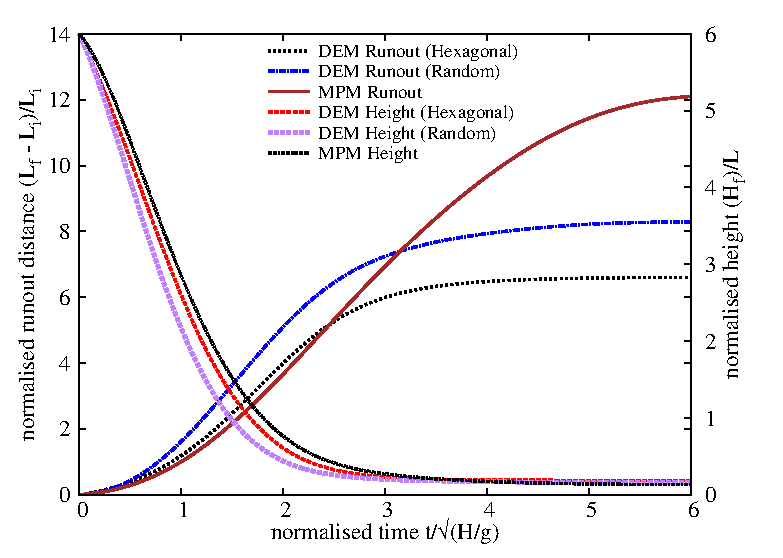
\includegraphics[width=\textwidth]{flowa6}
\caption{Flow evolution of a column with $a=6$}
\label{fig:flowa6}
\end{subfigure}
\caption{Flow evolution of granular column collapse (\textit{a} = 0.4 and 6).}
\label{fig:flow_column}
\end{figure}

\subsection{Energy dissipation mechanism}
\label{sec:energy}

The energy dissipation mechanism during collapse provides useful insights 
into the flow dynamics. In the case of small aspect ratios, the columns undergo 
no free fall. The spreading mainly results from the failure of the edges, while 
the top of the column remains essentially undisturbed in the central area. 
The amount of energy dissipated during the 
spreading $\delta E$ can be easily recovered using the simple shape of the 
final deposit and volume conservation (\cref{fig:volume_conservation}). The 
difference in potential energy between the initial and the final states gives

\begin{equation}
\delta E = \frac{1}{6} g \rho (L_f - L_0) H_0^2 \,,
\end{equation}

\begin{figure}
\centering
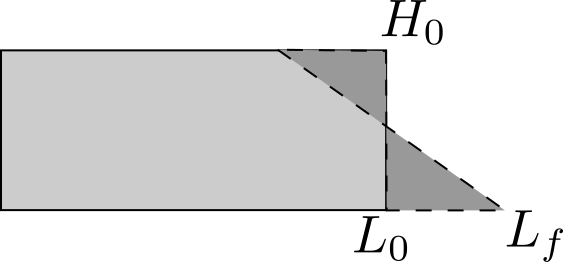
\includegraphics[width=0.7\textwidth]{volume_conservation}
\caption[Scheme of collapse for small aspect ratio columns.]{Scheme of collapse 
for small aspect ratio columns. The amount of 
energy $\delta E$ lost in the process can be evaluated
from the run-out distance $L_f - L_0$~\citep{Staron2007a}.}
\label{fig:volume_conservation}
\end{figure}

where $\rho$ is the density of the packing. It is assumed that this energy is 
dissipated by the work of frictional forces $W_{\mu}$ over the total run-out 
distance by the center of mass \textit{G} of the spreading 
material. The collapse involves two regions of dissipation: the amount of mass 
destabilised $\frac{1}{4}(L_f - 
L_0) H_0$ over two thirds of the run-out distance $2(L_f - L_0) / 3$ 
(considering
the triangular shape of the final deposit and the initial and the final 
positions of the centre of mass). The effective coefficient of friction $\mu_e$ 
characterises the mean dissipation in the flow. The work of friction forces is 

\begin{equation}
W_{\mu} = \frac{1}{6} \mu_e g \rho (L_f - L_0)^2 H_0 \,.
\end{equation}

Equating $\delta_E$ and $W_{\mu}$ gives $\mu_e (L_f - L_0) = H_0$. The scaling
of the runout leads directly to the relation $\mu_e = \lambda^{-1}$, where 
$\lambda$ is the numerical constant in the power-law relation between the 
run-out and the initial aspect ratio, which depends on the 
material properties. 
The amount of energy $\delta E$ dissipated 
during the spreading is compared with $W = N_p g m_p r_p$, where $N_p$ is the 
total number of grains, $m_p$ is their mass, and $r_p$ is the total horizontal 
distance run by each of them. The dissipation energy $\delta E$ 
is proportional to $W$.~\cite{Staron2007a} observed that the coefficient of 
proportionality gives a measure of the effective friction and 
observed a power law dependence between $\mu_e$ and internal friction angle 
$\mu$: $\mu_e=0.425\mu^{0.2}$. In this study, an effective friction angle 
$\mu_e$ of 21\si{\degree} is observed, which is very close to the critical 
state friction angle of 22\si{\degree} used in MPM simulations. The global 
effective friction angle obtained from the simple macroscopic 
energy-dissipation analysis matches the critical state friction used in MPM 
simulations. This proves that the energy dissipation mechanism modelled in a 
continuum sense as a frictional dissipation process captures the flow 
kinematics observed in DEM and experiments for short columns.

\Cref{fig:a04_energy} shows the time evolution of the normalised potential 
energy $(E_{p}/E_0)$ and kinetic energy $(E_{k}/E_0)$ for granular columns with 
an initial aspect ratio \textit{a} = 0.4. The normalised potential and kinetic 
energy 
are computed as
%
\begin{align}
E_p & = \sum\limits_{p=1}^{N_p}{m_p g h_p} \,, \\
E_{ki} & = \frac{1}{2}\sum\limits_{p=1}^{N_p}{m_p v_p^2} \,,
\end{align}
%
where $N_p$ is the total number of grains, $m_p$ is 
the mass of a grain \textit{p}, $h_p$ is the height and 
$v_p$ is the velocity of the grain \textit{p}. The cumulative dissipation 
energy is computed as
%
\begin{align}
\frac{E_d}{E_0} = 1 - \frac{E_k}{E_0} - \frac{E_p}{E_0} \,.
\end{align}
%
It can be observed that both MPM and DEM show similar energy dissipation 
mechanisms. The DEM simulation shows 3\% more potential energy dissipation in 
comparison with MPM simulations. This small difference in the potential energy 
is due to grain rearrangements. This shows the ability of the continuum 
approach to capture the flow kinematics of columns with small aspect ratios 
($a \le 
2.7$). 

The evolution of normalised kinetic and potential energy of a tall column 
collapse (\textit{a} = 6) are shown in~\cref{fig:a6_energy}. It can be 
observed that the initial potential energy stored in the 
grains is converted to kinetic energy which is dissipated as the granular 
material flows down. Three successive stages can be identified in the granular 
column collapse. In the first stage, similar to short columns, the flow is 
initiated by a well defined failure surface. However, the centre of gravity of 
the granular column is much 
higher than the top of the failure surface, which results in free fall of 
grains under gravity 
consuming the column along their way. In this stage which lasts for
$(t<0.8\tau_{c})$, the initial potential energy stored in the grains is 
converted into vertical motion. In the second stage, when the grains reach the 
vicinity of the failure surface, they undergo collisions with the bottom plane 
and the neighbouring grains, thus causing the flow to deviate along the 
horizontal direction releasing a large amount of kinetic energy gained during 
the free fall (\cref{fig:a6f}). In the third stage, the grains eventually 
leave the base area of the column and flow sideways~\citep{Lajeunesse2004}. As 
the process involves collective dynamics of all the grains, it is difficult 
to predict the exact trajectory of a grain, however, the overall dynamics can 
be explained. 


DEM simulations model both collisional and frictional dissipation processes 
during the collapse of tall columns. However, MPM simulations assume that the 
total initial potential energy stored in the system is completely dissipated 
through friction over the entire run-out distance, which results in longer 
run-out distance.~\Cref{fig:a6_energy} shows the evolution of normalised 
energies with time for MPM and DEM simulations. At the initial stage of 
collapse, characterised by free fall of grains under 
gravity, the DEM simulation, due to its particulate nature shows a rapid 
reduction in the potential energy in comparison with the MPM simulations, where 
the failure begins from the toe of the column. The continuum nature of the MPM 
simulations results in slower initiation of the collapse (\cref{fig:flowa6}). 
It can be also observed from~\cref{fig:a6_energy} that the dissipation of 
energy in MPM is 25\% less than in the DEM simulations. In order to understand 
the mechanism of energy dissipation, it is important to separate the 
contribution from the cumulative frictional and collisional parts. The 
frictional dissipation (basal and internal friction) observed in DEM is almost 
identical to the frictional dissipation observed in MPM (\cref{fig:a6_energy}). 
The difference in the dissipation energy is due to the collisional regime, 
which occurs at $0.8\tau_c$. The total dissipation and the frictional 
dissipation curves diverge around $0.8\tau_c$ where the grains near the 
vicinity of the failure surface undergo collisions with the bottom 
plane and the neighbouring grains resulting in collisional dissipation of the 
stored potential energy. DEM simulation show drop in the peak kinetic energy at 
$\approx0.8\tau_c$, which is at the beginning collisional dissipation stage. 
MPM lacks this collision dissipation mechanism, which results in longer run-out 
distances for columns with large aspect ratios. 

\begin{figure}[tbhp]
\centering
\begin{subfigure}[b]{0.975\textwidth}
\includegraphics[width=\textwidth]{a04_energy}
\caption{Energy evolution of a column with $a=0.4$.}
\label{fig:a04_energy}
\end{subfigure}
\\
\begin{subfigure}[b]{0.975\textwidth}
\centering
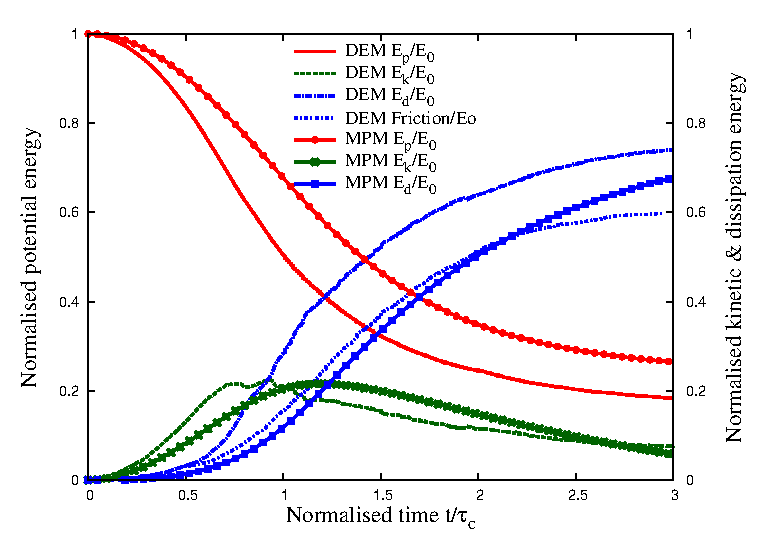
\includegraphics[width=\textwidth]{a6_energy}
\caption{Energy evolution of a column with $a=6$.}
\label{fig:a6_energy}
\end{subfigure}
\caption{Energy evolution of granular column collapse (\textit{a}=0.4 and 6).}
\label{fig:column_energy}
\end{figure}

The $\mu(I)$ rheology, discussed in~\cref{sec:muI}, describes the granular 
behaviour using a dimensionless number, called the \textit{inertial number I}, 
which is the ratio of inertia to the pressure forces. Small values of 
\textit{I} correspond to the critical state in soil mechanics and large values 
of \textit{I} corresponds to the fully collisional regime of kinetic theory. 
$\mu(I)$ rheology is adopted in MPM simulations to understand the 
characteristics of the flow regime. The Mohr-Coulomb model was used along with 
$\mu(I)$ rheology. The friction angle is changed according to a friction 
law~\citep{DaCruz2005} that is dependent on the inertial number \textit{I} as 
$\mu = \mu_{min} + b \mathit{I}$, where $\mu_{min} = 0.22$ and \textit{b} = 
1.~\Cref{fig:flow_muI} shows the flow evolution of granular column collapse for 
aspect ratios \textit{a} of 0.4 and 6 using $\mu(I)$ rheology. For short 
columns, the evolution of flow based on $\mu(I)$ rheology is identical to the 
MPM simulation using Mohr-Coloumb model. However, for tall columns, $\mu(I)$ 
rheology evolves at the same rate as the DEM simulations up to $t = 0.8\tau_c$, 
after which the MPM simulation continues to accelerate due to lack of 
collisional dissipation, while the DEM simulation decelerates with time. 

\begin{figure}[tbhp]
\centering
\begin{subfigure}[b]{0.975\textwidth}
\includegraphics[width=\textwidth]{flowa04muI}
\caption{Flow evolution of a column with $a=0.4$ using $\mu(I)$ rheology.}
\label{fig:flowa04muI}
\end{subfigure}
\\
\begin{subfigure}[b]{0.975\textwidth}
\centering
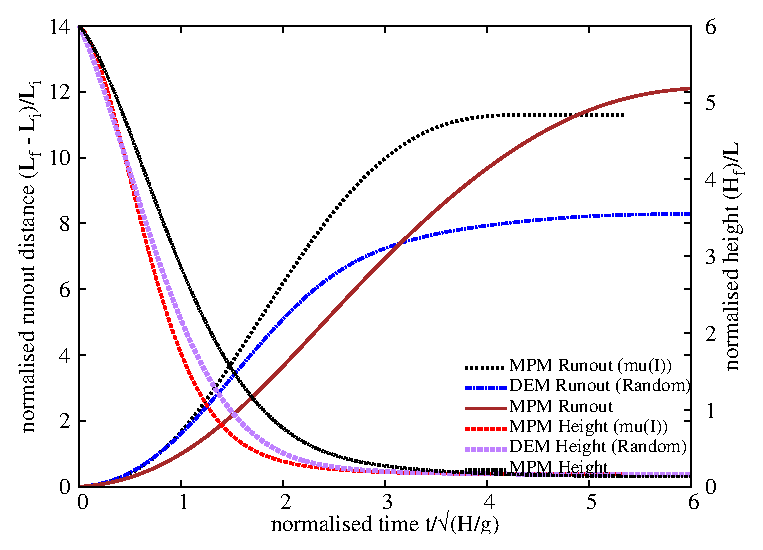
\includegraphics[width=\textwidth]{flowa6muI}
\caption{Flow evolution of a column with $a=6$ using $\mu(I)$ rheology.}
\label{fig:flowa6muI}
\end{subfigure}
\caption{Flow evolution of granular column collapse using $\mu(I)$ rheology 
(\textit{a}=0.4 and 6).}
\label{fig:flow_muI}
\end{figure}

~\Cref{fig:muI} shows that the short column attains a maximum inertial 
number of 0.012, which is in the dense granular flow regime, inertial number 
$\approx10^{-3} < I < 0.1$~\citep{DaCruz2005}. However for the tall 
column, the maximum inertial number $I\approx0.04$ is still within the 
dense granular flow regime. DEM simulations, however, showed a collisional 
regime that has inertial numbers higher than 0.1. This shows that continuum 
approach using frictional laws are able to capture the flow kinematics at small 
aspect ratios, however they are unable to precisely describe the flow dynamics 
of tall columns, which is characterised by an initial collisional regime. This 
suggests that triggering mechanisms play a crucial role in the case of 
modelling the natural flows. This stresses the necessity of accounting for 
initiation mechanisms while modelling the run-out behaviour 
using continuum approaches to predict realistic granular flow behaviour. The 
role of the initiation mechanism on the run-out behaviour and the ability of 
MPM in modelling transient flows that does not involve collision are 
investigated in~\cref{sec:slope}. The initial material property has a 
significant influence on the run-out behaviour. This aspect has attracted less 
research. In the next section, 2D DEM simulations are performed to understand 
the influence of initial grain properties on the collapse. This gives us a 
better understanding of the input parameters required in the continuum 
modelling. 

\begin{figure}[tbhp]
\centering
\includegraphics[width=\textwidth]{muI}
\caption{MPM simulation of evolution of inertial number with time for columns 
with $a=0.4$ and 
$a=6$.}
\label{fig:muI}
\end{figure}

\section{Role of initial grain properties on the collapse of granular columns}

The role of material properties and the distribution of mass in the system have 
been shown to have a non-trivial influence on the flow kinematics and the 
internal flow structure. Hence it is important to understand the role of 
initial packing density on the run-out behaviour in the case of granular column 
collapse.~\citet{Lube2005} observed that the run-out distance scales with the 
initial aspect ratio of the column, independent of the material properties. The 
run-out evolution after the initial transition regime is a frictional 
dissipation process, and the lack of influence of material properties on the 
run-out behaviour is inconsistent with frictional dissipation in continuum 
modelling of granular flow behaviour.~\citet{Balmforth2005} observed that the 
material properties have almost no influence on the exponent of the normalised 
run-out as a function of the initial aspect ratio. The numerical constant of 
proportionality, however, showed clear material dependence. This corroborates 
the conclusions of~\citet{Lajeunesse2004} and refutes that 
of~\citet{Lube2005}.~\citet{Daerr1999} also observed strong influence of 
initial packing density and the internal structure on the behaviour of 
granular flows. 


It should be noted that the collapse experiment is highly transient and no 
clear stationary regime is observed. On the contrary, the acceleration and the 
deceleration phases cover nearly the whole duration of the spreading. This 
makes it difficult to analyse the flow structure and its relation with other 
characteristic of the system. The knowledge of the final run-out is not a 
sufficient characterization of the deposit; one also needs to know how the mass 
is distributed during the flow to understand the dynamics and the dissipation 
process. This is expected to be true in natural contexts as well as in 
experiments. While the inter-grain friction does not affect the early vertical 
dynamics, nor the power-law dependence, it controls the effective frictional 
properties of the flow, and its internal structure~\citep{Staron2007a}. It is 
interesting to note that the details of the structure of the flow do not 
influence the final run-out dependence, and thus seem to play a marginal role 
in the overall behaviour of the spreading. This could explain why a simple 
continuum model with a frictional dissipation could reproduce the run-out 
scaling for columns with small aspect ratios. 

Most research has been focussed on the run-out behaviour of mono-disperse 
grain sizes. However, the influence of initial packing density and 
poly-dispersity have attracted less interest. In the present study, DEM 
simulations of collapse of loose (79\% packing density) and dense (83\% 
packing density) granular columns with an initial aspect ratio \textit{a} of 
0.8 are performed to understand the influence of material properties on the 
run-out behaviour. The evolution of normalised run-out with time for two 
different initial packing densities are presented 
in~\cref{fig:runout_height_dense_r18}. At the initial 
stage of collapse $t=\tau_c$, the flow evolution is identical in both dense and 
loose conditions. However, the dense column flows for 30\% longer than the 
loose columns. Both the columns come to rest at around $t = 4\tau_c$. The 
columns, however, show similar evolution of the normalised height. This shows 
that only a part of the column is destabilised during the collapse.
\begin{figure}[h]
\centering
\includegraphics[width=0.9\textwidth]{runout_height_dense_r18}
\caption{Effect of density on the run-out evolution $a = 0.8$.}
\label{fig:runout_height_dense_r18}
\end{figure}

\begin{figure}[h]
\centering
\includegraphics[width=0.9\textwidth]{voro_r18}
\caption{Evolution of local packing density with time $a = 0.8$.}
\label{fig:voro_r18}
\end{figure}

\Cref{fig:Energy_density_r18} shows the evolution of potential and kinetic 
energy with time. Similar potential energy evolution in both dense and loose 
conditions reveals that there is no change in the overall mechanism of 
collapse. The dense condition has a slightly higher peak kinetic energy than 
the loose column. In the free-fall phase, the dense column shows a steeper 
increase in the horizontal kinetic energy in comparison to the loose column. 
This indicates that the dense granular mass is pushed farther away more quickly 
than with the loose column. A loose column exhibits higher vertical kinetic 
energy which may be due to particle rearrangement resulting in densification of 
the granular mass.~\Cref{fig:voro_r18} shows that the loose sample densifies as 
the flow evolves. Both dense and loose granular columns dilate during the 
initial stage of collapse, this is due to grains experiencing shear along the 
shear-failure surface. In both cases, the granular mass attains similar packing 
density at the end of the flow. The dense granular column dilates, while the 
loose column compacts to achieve the same critical density. The dense condition 
has higher mobilised potential energy during the initial stage of collapse, 
which yields higher horizontal kinetic energy for the flow. However in loose 
conditions, a higher proportion of the available energy is lost during 
compaction. This behaviour in addition to higher mobilised potential energy 
results in longer run-out distance in dense granular 
column.~\citet{Lajeunesse2004} observed that the flow comes to rest at around 
$3\tau_c$, but the grains continue to re-arrange until $6\tau_c$. Similar 
behaviour is observed in DEM simulations.

\begin{figure}[tbhp]
\centering
\begin{subfigure}[b]{0.75\textwidth}
\centering
\includegraphics[width=\textwidth]{Energy_dense_r18}
\caption{Evolution of potential and kinetic energy}
\label{fig:Energy_dense_r18}
\end{subfigure}
\\
\begin{subfigure}[b]{0.75\textwidth}
\centering
\includegraphics[width=\textwidth]{KExy_dense_r18}
\caption{Effect of kinetic energy}
\label{fig:KExy_dense_r18}
\end{subfigure}
\caption{Effect of density on the energy evolution $a = 0.8$.}
\label{fig:Energy_density_r18}
\end{figure}

In order to remove the effect of crystallisation on the run-out behaviour, a 
highly poly-disperse sample ($r = d_{max}/d_{min} = 6)$ is used. 
The flow kinematics of a dense (relative density $D_r = 74\%$) and a loose 
($D_r = 22\%$) granular column with aspect ratio of 0.8 is 
studied.~\Cref{fig:runout_height_dense_r6} shows the evolution of the 
normalised run-out with time for dense and loose granular columns with an 
initial aspect ratio of 0.4. Similar to 
the previous case, the dense granular column exhibits longer run-out distance 
(\cref{fig:runout_height_dense_r6}).~\Cref{fig:Energy_dense_r6} show the 
evolution of energy with time for dense and loose conditions. The peak kinetic 
energy in the dense condition is $\sim 20\%$ higher than the loose 
condition. Due to compaction of grains in loose condition, almost 20\% of the 
normalised initial potential energy available for the collapse is lost in 
densification due to grain rearrangements in comparison to the dense 
condition (\cref{fig:Energy_voro_r6}). The compaction of grains in loose 
column and the dilation in dense column results in significantly different flow 
structure, especially at the flow front (\cref{fig:density_r6}). As the loose 
column densifies, more granular mass is pushed to the flow front resulting in 
higher vertical effective stress. The loose column exhibits a more parabolic 
final deposit profile in comparison to the dense column, which shows a 
triangular deposit at the front.

\begin{figure}[tbhp]
\centering
\includegraphics[width=0.8\textwidth]{runout_height_dense_r6}
\caption{Effect of density on the run-out evolution $a = 0.8$ (poly-dispersity 
\textit{r} = 6).}
\label{fig:runout_height_dense_r6}
\end{figure}


\begin{figure}[bhp]
\centering
\begin{subfigure}[b]{\textwidth}
\centering
\includegraphics[width=\textwidth]{dense_a08_r6_final}
\caption{Dense initial packing}
\label{fig:dense_a08_r6_final}
\end{subfigure}
\\
\begin{subfigure}[b]{\textwidth}
\centering
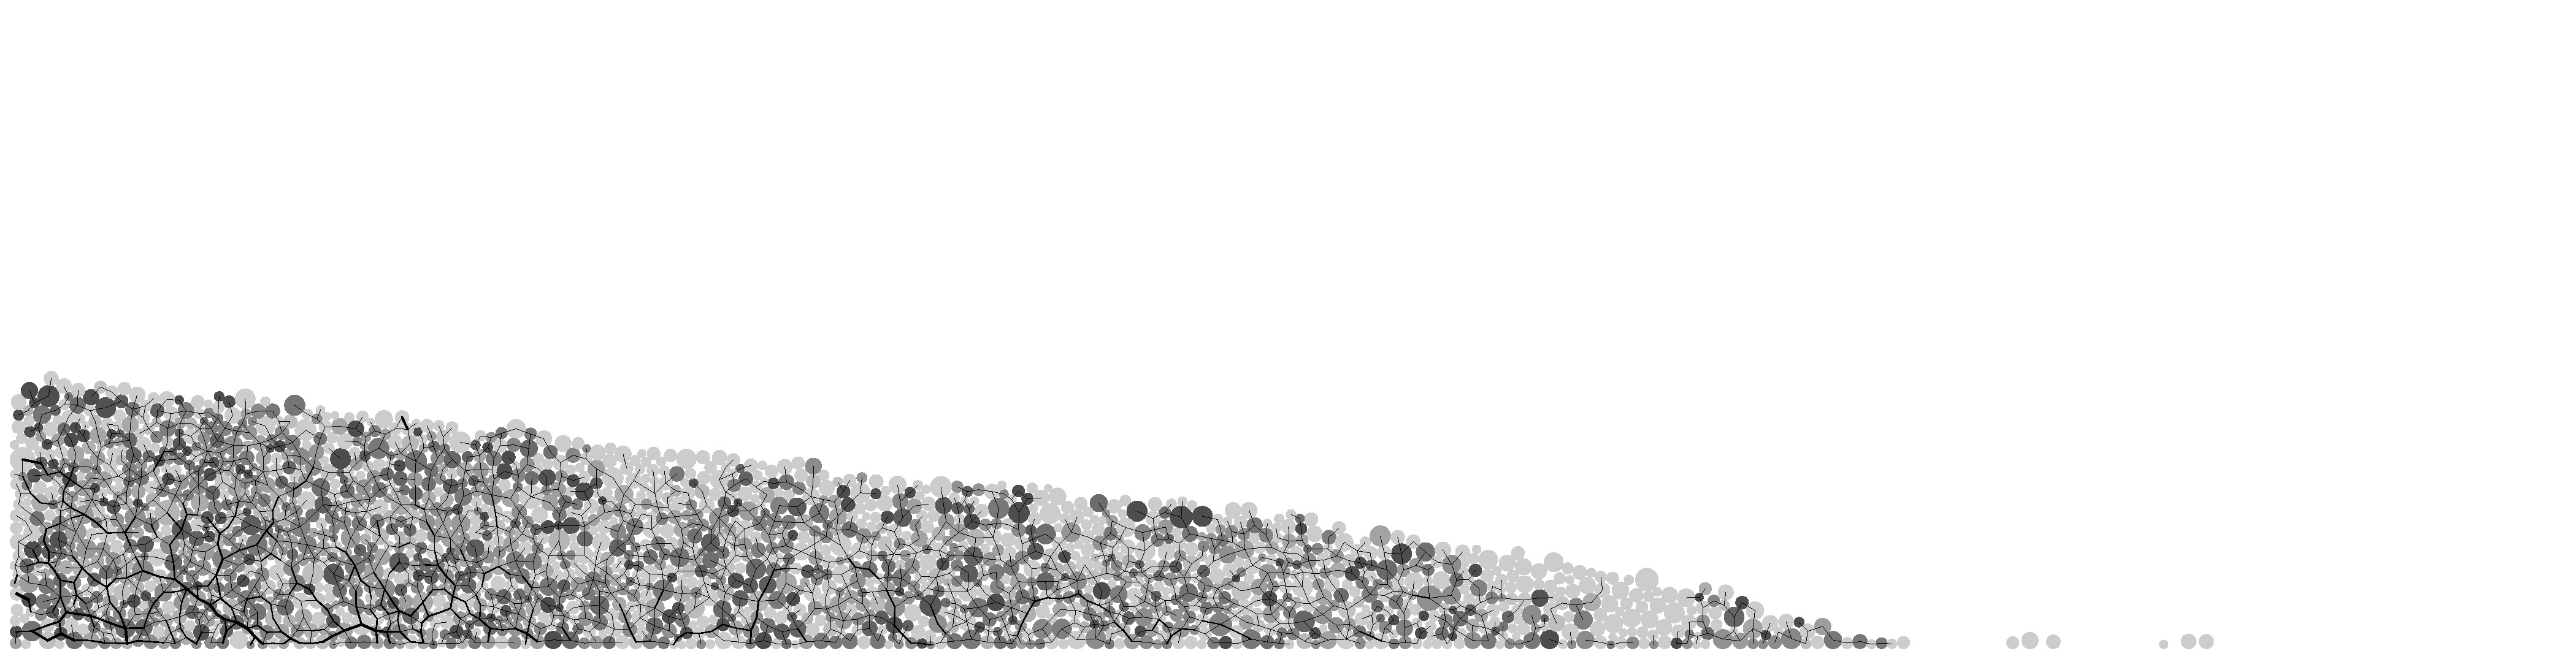
\includegraphics[width=\textwidth]{loose_a08_r6_final}
\caption{Loose initial packing}
\label{fig:loose_a08_r6_final}
\end{subfigure}
\caption{Snapshots of granular column collapse at $t = 6 \tau_c$ (\textit{a} = 
0.8).}
\label{fig:density_r6}
\end{figure}


\begin{figure}[tbhp]
\centering
\begin{subfigure}[b]{0.75\textwidth}
\centering
\includegraphics[width=\textwidth]{Energy_dense_r6}
\caption{Evolution of potential and kinetic energy}
\label{fig:Energy_dense_r6}
\end{subfigure}
\\
\begin{subfigure}[b]{0.75\textwidth}
\centering
\includegraphics[width=\textwidth]{voro_r6}
\caption{Evolution of packing density}
\label{fig:voro_r6}
\end{subfigure}
\caption{Effect of density on the evolution of energy and packing fraction $a = 
0.8$ (poly-dispersity `r' = 6).}
\label{fig:Energy_voro_r6}
\end{figure}

In short columns, only a part of the granular column above the failure surface 
participates in the flow. However, it appears that the collapse for 
large aspect ratios mixes two very different dynamics: the first stage 
shows a large vertical acceleration, while the second stage 
consists of a ``conventional'' horizontal granular flows. This section 
investigates the effect of density 
on the run-out behaviour of tall columns. Similar to short 
columns, the dense granular column with an aspect ratio of 6 shows higher 
run-out distance in comparison to the loose condition. The dense granular 
column flows almost twice as much as that of the loose column. Unlike short 
columns, the evolution of run-out is different even at the initial stage of the 
collapse. The dense granular column, which has higher initial potential energy 
shows a rapid increase in the run-out due to free-fall and higher mobilised 
potential energy. During this stage of collapse, the dense granular column has 
15 \% higher normalised kinetic energy available for the horizontal push. This 
results in a longer run-out distance for a dense granular column in comparison 
to an initially loose granular column.

\begin{figure}[tbhp]
\centering
\begin{subfigure}[b]{0.95\textwidth}
\includegraphics[width=\textwidth]{runout_height_dense_a6}
\caption{Effect of density on run-out evolution.}
\label{fig:runout_height_dense_a6}
\end{subfigure}
\\
\begin{subfigure}[b]{0.95\textwidth}
\centering
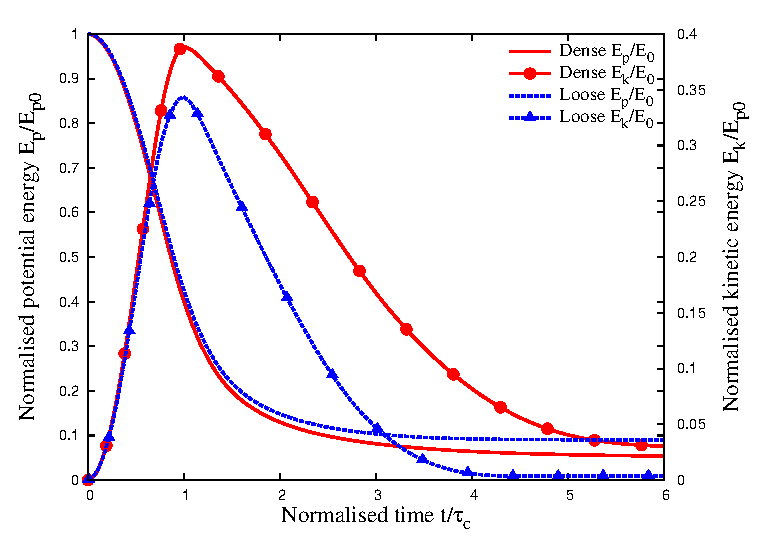
\includegraphics[width=\textwidth]{Energy_dense_a6}
\caption{Effect of density on energy evolution.}
\label{fig:Energy_dense_a6}
\end{subfigure}
\caption{Effect of density on the run-out behaviour and energy evolution $a = 
0.6$.}
\label{fig:Density_a6}
\end{figure}

The initial packing fraction and the distribution of kinetic energy in the 
system has a significant influence on the flow kinematics and the run-out 
behaviour. The next section will discuss the influence of triggering mechanism 
and the distribution of the kinetic energy in the granular system on the 
run-out behaviour.  

%\clearpage

\section{Slopes subjected to horizontal excitation}
\label{sec:slope}
Transient granular flows occur very often in nature. Well-known examples are 
rockfalls, debris flows, and aerial and submarine avalanches. In the 
geotechnical context, transient movements of large granular slopes 
is a substantial factor of risk due to their destructive force and the 
transformations they may produce in the landscape. Natural granular flows 
may be triggered as a result of different processes such as gradual 
degradation induced by weathering or chemical reactions, liquefaction and 
external forces such as earthquakes. Most contemporary research on granular 
materials deals with steady-state flow. Transients and inhomogeneous 
boundary conditions are much less amenable to observation and analysis, and 
have thus been less extensively studied despite their primary importance in 
engineering practice. In most cases of granular flow, an initially static pile 
of grains is disturbed by external forces, it then undergoes an abrupt 
accelerated motion and spreads over long distances before relaxing to a new 
equilibrium state. The kinetic energy acquired during destabilisation is 
dissipated by friction and inelastic collisions.

This section investigates the ability of MPM, a continuum approach, to 
reproduce the evolution of a granular pile destabilised by an external energy 
source. In particular, a central issue is whether the power-law dependence of 
run-out distance and time observed with respect to the initial geometry or 
energy can be reproduced by a simple Mohr-Coulomb plastic behaviour for 
granular slopes subjected an horizontal excitation. The effects of different 
input parameters, such as the distribution of energy and base friction, on the 
run-out kinematics are studied by comparing the data obtained from DEM and MPM 
simulations.

\subsection{Numerical set-up}
\label{sec:num}

The DEM sample was composed of $\sim13000$ disks with a uniform distribution of 
diameters by volume fractions ($d_{max} = 1.5 d_{min}$). The mean grain 
diameter and mass are $d\simeq 2.455 $~\si{\mm} and $m\simeq 0.0123$~\si{\kg}, 
respectively. The grains are first poured uniformly into a rectangular box of 
given width and then the right-hand side wall is shifted far to the right 
to allow the grains to spread. A stable granular slope of 13.2~\si{\degree} is 
obtained when all grains come to rest; see~\cref{fig:slope_configuration}. This 
procedure leads to a mean packing fraction $\simeq 0.82$. Soil grains with a 
mean density of 2600~\si{\kg\per\m\cubed} and internal friction coefficient of 
0.4 between grains are considered.

\begin{figure}[tbhp]
\includegraphics[width=0.95\textwidth]{slope_configuration}
\caption{Initial geometry and dimensions of the pile subjected to a horizontal 
excitation.}
\label{fig:slope_configuration}
\end{figure}


The initial static pile was set into motion by applying a horizontal
gradient velocity $v_{0x}(y) = k (y_{max} - y)$ with $k>0$. The evolution of 
the pile geometry and the total kinetic energy as a function of the initial 
input energy $E_0$ is studied. The run-out distance $L_f$ is the distance of 
the rightmost grain, which is still in contact with the main mass when the pile 
comes to rest. The run-out will be normalised by the initial length $L_0$ of 
the pile, as in the experiments of collapsing columns. The total run-out 
duration $t_f$ is the time taken by the pile to reach its final run-out 
distance $L_f$.

For grain-scale simulations, classical DEM and Contact Dynamics approaches were 
used. This research was done in collaboration with Patrick Mutabaruka, 
University of Montpellier, who performed Contact Dynamics (CD) simulations that 
are presented in this section. A detailed description of the Contact Dynamics 
method can be found in \cite{Moreau1993,Jean1999,Radjai2009,Radjai2011}. 
The CD method is based on implicit time integration of the equations of motion 
and a non-smooth formulation of mutual exclusion and dry friction between 
particles. The CD method requires no elastic repulsive potential and no 
smoothing of the Coulomb friction law for the determination of forces. 
For this reason, the simulations can be performed with large time steps 
compared to discrete element simulations. The unknown variables are particle 
velocities and contact forces, which are calculated at each time step by taking 
into account the conservation of momenta and the constraints due to mutual 
exclusion between particles and the Coulomb friction. An iterative 
algorithm based on a non-linear Gauss-Seidel scheme is used. The only 
contact parameters within the CD method are the friction coefficient $\mu$, the 
normal restitution coefficient $\varepsilon_n$ and the tangential restitution 
coefficient $\varepsilon_t$ between grains. 

In MPM simulations, the material point spacing is adopted to be the same as the 
mean grain diameter in DEM. A mesh size of 0.0125m is adopted with 25 material 
points per cell. The effect of mesh size and the number of material points per 
cell is investigated in~\cref{sec:MPM_points_per_cell}. The initial 
configuration of the slope in MPM is shown in~\cref{fig:MPM_Initial_PIC_Slope}. 
Frictional boundary conditions are applied on the left and the bottom 
boundaries by applying constraints to the nodal acceleration. The initial 
vertical stress of the granular pile in equilibrium, before the horizontal 
excitation, in the MPM simulation is shown in~\cref{fig:MPM_Stress_Slope}. The 
distribution of the initial gradient horizontal excitation energy of 50~\si{J} 
on the granular pile is shown in~\cref{fig:MPM_Velocity_Slope}. The 
Mohr-Coulomb model with no dilation is used to simulate the continuum behaviour 
of the granular pile. Periodic shear tests using CD 
(\cref{fig:Sxy_vs_Syy_Slope}), reveals a macroscopic friction coefficient of 
0.22. The evolution of inertial number with friction is presented 
in~\cref{fig:mu_vs_I}. 

\begin{figure}[tbhp]
\centering
\begin{subfigure}[t]{0.75\textwidth}
\centering
\includegraphics[width=0.95\textwidth]{MPM_Initial_PIC_Slope}
\caption{Initial configuration of material points per cell. 25 material points 
per cell. Cell size of 0.0125m.}
\label{fig:MPM_Initial_PIC_Slope}
\end{subfigure} \\
%
\begin{subfigure}[t]{0.95\textwidth}
\centering
\includegraphics[width=0.95\textwidth]{MPM_Stress_Slope}
\caption{Initial stress in MPM}
\label{fig:MPM_Stress_Slope}
\end{subfigure} \\
%
\begin{subfigure}[t]{0.95\textwidth}
\centering
\includegraphics[width=0.95\textwidth]{MPM_Velocity_Slope}
\caption{Initial horizontal velocity for a pile subjected to a horizontal 
velocity of 50J.}
\label{fig:MPM_Velocity_Slope}
\end{subfigure}
\caption{Initial configuration for the MPM simulation of a pile subjected to 
horizontal velocities.}
\label{fig:MPM_Slope_setup}
\end{figure}


\begin{figure}[tbhp]
\centering
\begin{subfigure}[t]{0.475\textwidth}
\includegraphics[width=0.95\textwidth]{Sxy_vs_Syy_Slope}
\caption{Evaluation of the critical state friction angle.}
\label{fig:Sxy_vs_Syy_Slope}
\end{subfigure}
%
\begin{subfigure}[t]{0.475\textwidth}
\includegraphics[width=0.95\textwidth]{mu_vs_I}
\caption{Evolution of Inertial number with friction $\mu$.}
\label{fig:mu_vs_I}
\end{subfigure}
\caption{Periodic shear test using CD~\citep{Mutabaruka2013}.}
\label{fig:Shear_Test_Slope}
\end{figure}

The natural units of the system 
are the mean grain diameter $d$, the mean grain 
mass $m$ and acceleration due to gravity $g$. For this reason, the length 
scales are normalised by $d$, time by $(d/g)^{1/2}$, velocities by $(gd)^{1/2}$ 
and energies by $mgd$. 


\subsection{Effect of mesh size and number of material points per cell}
\label{sec:MPM_points_per_cell}

The accuracy of MPM simulations largely depends on the number of material 
points representing the continuum. MPM utilises a grid to compute the 
deformation of a continuum, hence the size of the cells affects the accuracy 
of the results. Generally in MPM, the number of particles per cell controls 
the accuracy of the simulation.~\citet{Guilkey2003} recommends higher particle 
density, such as 4 particles per cell, for large deformation problems. Very low 
particle density will result in non-physical opening of cracks in large 
deformation simulations. However, a higher value of particle density affects 
the computational time. 

\citet{Abe2013} observed that for a coarse mesh, the numerical error 
decreases with an increase in the number of material points per cell. In 
contrast, they observed an opposite trend for fine meshes. The influence of 
numerical noise due to particles crossing the background mesh is not observed 
in coarse meshes.~\citet{Coetzee2005} also found that the numerical error 
decreases with increase in mesh refinement.

In the present study, the effect of mesh size and the number of material points 
per cell on the run-out behaviour of a static slope subjected to a horizontal 
excitation is investigated. A mesh size of 0.0125~\si{\m} is adopted. The 
number of material points per cell (PPC) is varied as 4, 16, 25, 36, 64, 81 and 
100.

The effect of the number of material points on the run-out behaviour is 
presented in~\cref{fig:Runout_MPM}. At a low input energy of 50~\si{\J}, 4 and 
16 material points per cell result in a longer run-out distance, whereas the 
run-out distance converges when the number of PPC is more than 25. However, at 
a high input energy of 500~\si{J}, both 4 and 16 PPC predict almost the same 
run-out distance, but the run-out is higher than the run-out predicted with 
more than 25 material points per cell. 

\begin{figure}[tbhp]
\centering
\begin{subfigure}[b]{0.95\textwidth}
\includegraphics[width=\textwidth]{Runout_50}
\caption{$E_0=12.7mgd$}
\label{fig:Runout_50}
\end{subfigure}
\\
\begin{subfigure}[b]{0.95\textwidth}
\centering
\includegraphics[width=\textwidth]{Runout_500}
\caption{$E_0=152mgd$}
\label{fig:Runout_500}
\end{subfigure}
\caption{Evolution of run-out with time for varying material points per cell 
for a slope subjected to a horizontal velocity.}
\label{fig:Runout_MPM}
\end{figure}

The evolution of the granular pile during the initial stage of flow is shown 
in~\cref{fig:MPM_50ppc} for different numbers of material points per cell. At 
low input energy, fewer material points per cell results in a larger separation 
of the spreading mass from the left wall. Distinct shear bands can be observed 
for more than 16 PPC. The flow structure remains unchanged with increase in PPC 
of more than 25. At a higher input energy
(\cref{fig:MPM_500ppc}), almost all cases predict similar flow structure, 
except in the case of 4 PPC.

\begin{figure}[tbhp]
\centering
\includegraphics[height=\textheight]{MPM_50ppc}
\caption{Effect of number of material points on cell on the run-out behaviour 
$E_0=12.7mgd$. 
Velocity profile (\si{\m/\s}) of granular pile subjected to gradient horizontal 
loading.}
\label{fig:MPM_50ppc}
\end{figure}


\begin{figure}[tbhp]
\centering
\includegraphics[height=\textheight]{MPM_500ppc}
\caption{Effect of number of material points on cell on the run-out behaviour 
$E_0=152mgd$. 
Velocity profile (\si{\m/\s}) of granular pile subjected to gradient horizontal 
loading.}
\label{fig:MPM_500ppc}
\end{figure}

\Cref{fig:KE_MPM} shows the evolution of kinetic energy with time for varying 
number of material points per cell. At low input energy, the horizontal kinetic 
energy evolution is identical for all cases. A slightly quicker run-out 
evolution during the spreading phase can be observed for the case of 4 PPC.  
However, increase in the number of material points per cell significantly 
affects the evolution of the vertical kinetic energy $E_{ky}$. At low energy, a 
large proportion of the input energy is dissipated in the destabilisation 
process. This results in material points falling behind the spreading mass to 
the fill the cavity. Fewer material points per cell results in cell-crossing 
noise as the material points filling the cavity experience free-fall due to 
gravity. The effect of cell-crossing noise can be seen in the oscillation of 
vertical kinetic energy for fewer material points per cell. However, at high 
input energy, most of the input velocity is dissipated during the spreading 
process. This means that only a small fraction of energy is available in the 
vertical component resulting in almost identical behaviour for all cases. Four 
material points per cell predicts a higher peak vertical kinetic energy in 
comparison with other case and unlike the low energy case, no oscillations are 
observed for high input energy.

\begin{figure}[tbhp]
\centering
\begin{subfigure}[b]{0.95\textwidth}
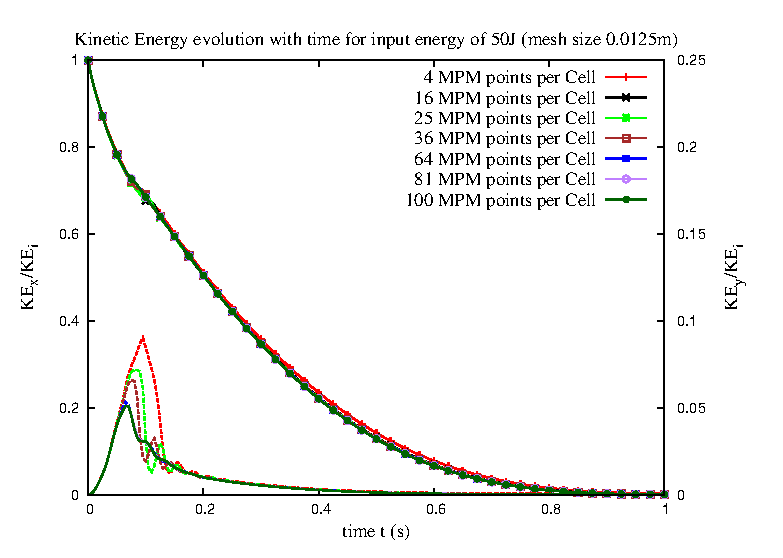
\includegraphics[width=\textwidth]{KE_50}
\caption{$E_0=12.7mgd$}
\label{fig:KE_50}
\end{subfigure}
\\
\begin{subfigure}[b]{0.95\textwidth}
\centering
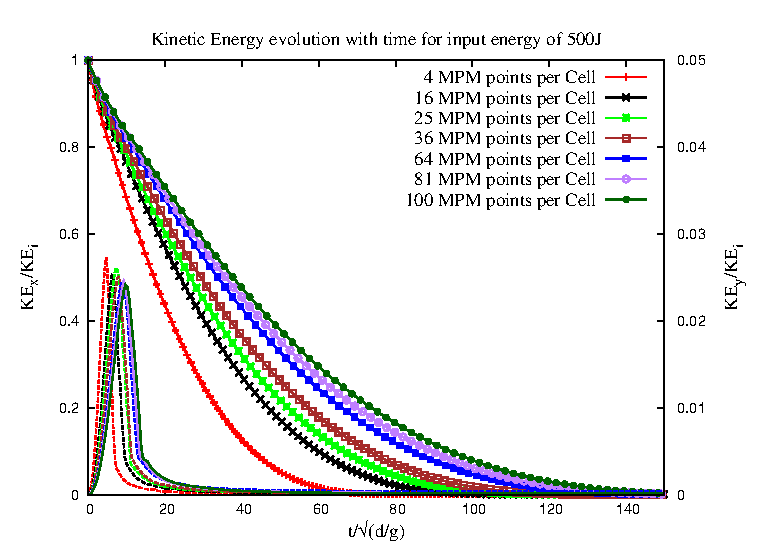
\includegraphics[width=\textwidth]{KE_500}
\caption{$E_0=152mgd$}
\label{fig:KE_500}
\end{subfigure}
\caption{Evolution of kinetic with time for varying material points per cell 
for a slope subjected to a horizontal excitation.}
\label{fig:KE_MPM}
\end{figure}

The effect of mesh size on the flow kinematics is studied by comparing two mesh 
sizes: 0.01~\si{\m} and 0.0125~\si{\m} (\cref{fig:MPM_Size_Effect}). It can 
be observed that the run-out distance converges with an increase in the number 
of material points per cell in both cases. Less than ~1\% difference in the 
run-out distance is observed between a mesh size of 0.0125~\si{\m} and 
0.01~\si{\m}. The final run-out duration is almost unaffected by the increase 
in the number of material points per cell. 
 

\begin{figure}[tbhp]
\centering
\begin{subfigure}[b]{0.95\textwidth}
\includegraphics[width=\textwidth]{50}
\caption{$E_0=12.7mgd$}
\label{fig:50}
\end{subfigure}
\\
\begin{subfigure}[b]{0.95\textwidth}
\centering
\includegraphics[width=\textwidth]{500}
\caption{$E_0=152mgd$}
\label{fig:500}
\end{subfigure}
\caption{Evolution of run-out and duration of flow  for varying material points 
per cell for a slope subjected to a horizontal excitation.}
\label{fig:MPM_Size_Effect}
\end{figure}

This shows that the run-out distance is affected by the number of material 
points per cell. However, the duration of the run-out is independent of the 
number of material points per cell. The computation time increases with 
increase in the number of material points per cell and decrease in the mesh 
size. However, the run-out distance converges with increase in number of 
material points per cell. Hence, an optimum number of 25 material points per 
cell is adopted in this case. In summary, for conducting a successful MPM 
analysis, a careful selection of the mesh size and the number of particles is 
necessary.


%-------------------------------------------------------------------------------
\subsection{Evolution of pile geometry and run-out}
\label{sec:evolution}

\Cref{fig:Gradient_Slope_Profile_200J} shows the initial evolution of the 
granular slope subjected to an initial horizontal energy $E_0 = 61$ (in 
dimensionless units) using MPM. As the granular slope is sheared along the 
bottom, the shear propagates to the top leaving a cavity in the vicinity of the 
left wall. This cavity gets partially filled as the granular mass at the top 
collapse behind the flowing mass due to inertia. Similar behaviour is observed 
during the initial stages of the flow evolution using CD technique 
(\cref{fig:Gradient_Slope_CD_200J}). Due to inertia, the grains at the top 
of the granular heap roll down to fill the cavity, while the pile continues to 
spread. 

\begin{figure}[tbph]
\centering
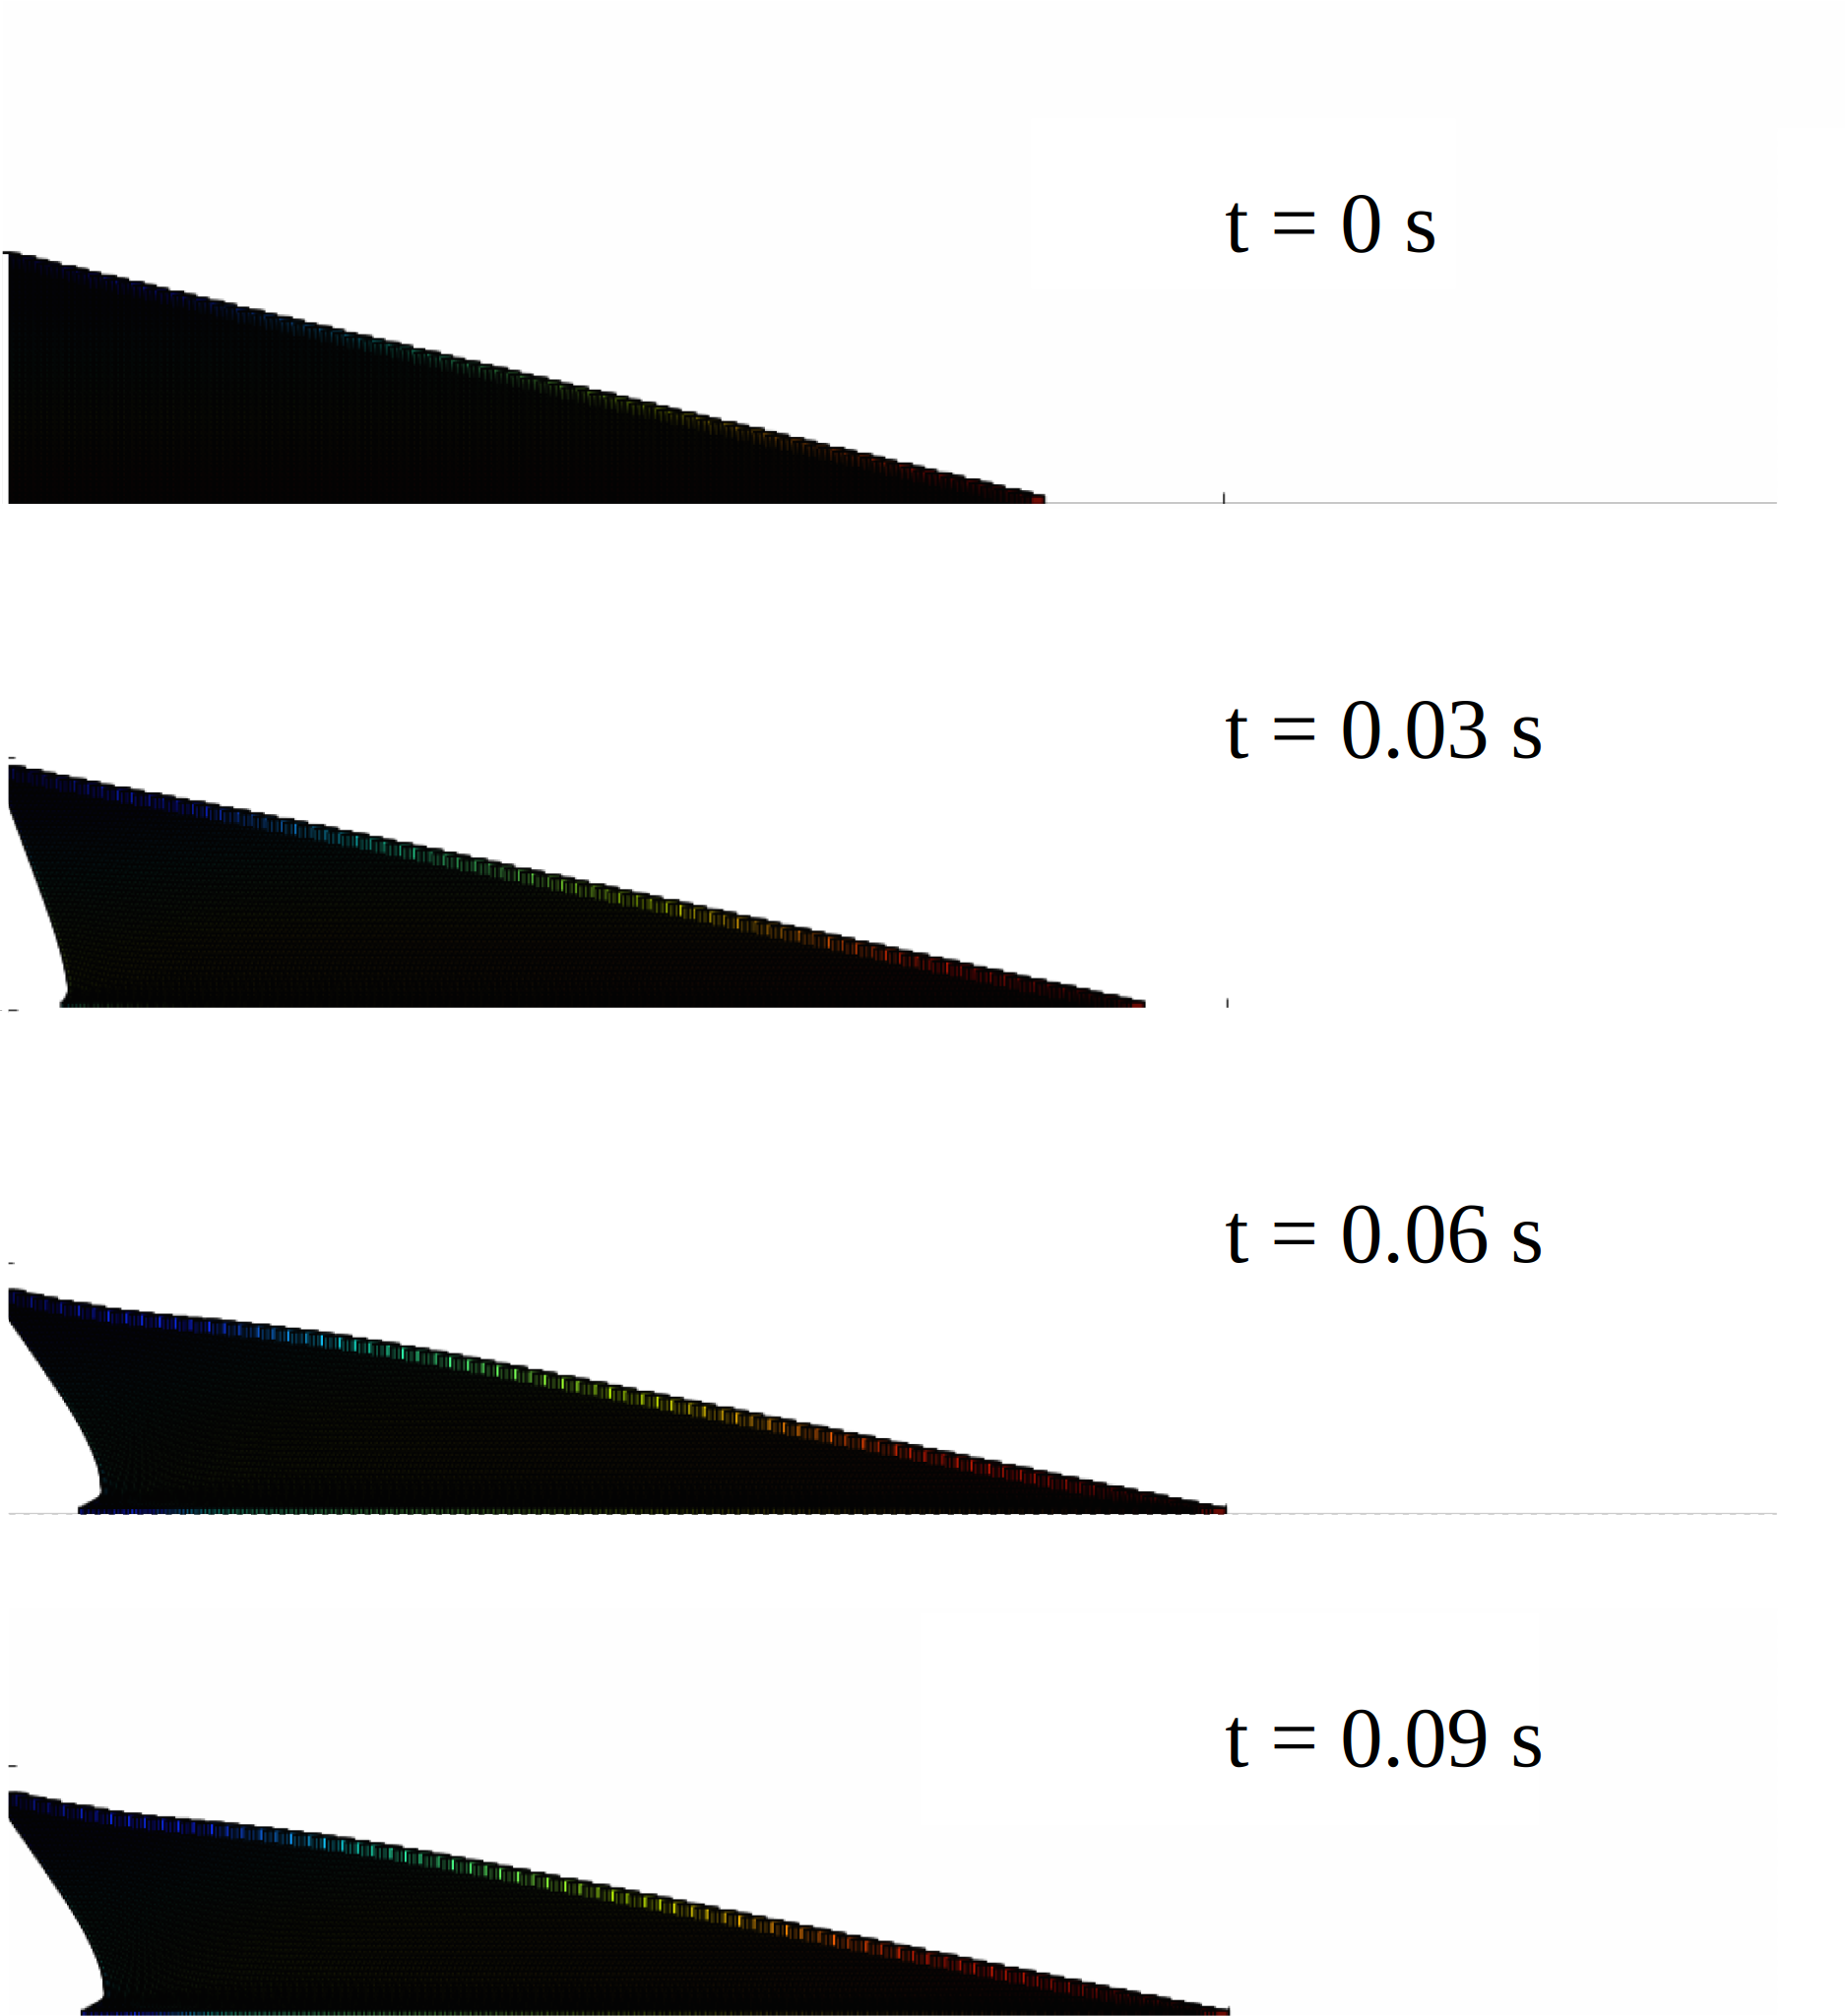
\includegraphics[width=\textwidth]{Gradient_Slope_Profile_200J}
\caption{MPM simulation of the initial stages of granular pile subjected to a 
gradient horizontal energy.}
\label{fig:Gradient_Slope_Profile_200J}
\end{figure}

\begin{figure}
\centering
\includegraphics[width=\textwidth]{Gradient_Slope_CD_200J}
\caption{CD simulation of the initial stages of granular pile subjected to a 
gradient horizontal energy.~\citep{Mutabaruka2013}.}
\label{fig:Gradient_Slope_CD_200J}
\end{figure}

The flow involves a transient phase with a change in the geometry of the pile 
followed by continuous spreading. The gradient of input energy applied to the 
granular slope mimics a horizontal quake. Despite the creation 
of a cavity behind the flowing mass, the granular heap remains in 
contact with the left wall irrespective of the input 
energy.~\Cref{fig:Runout_Eo_MPM_CD_DEM} shows the normalised run-out distance 
$(L_f - L_0)/L_0$ and total run-out time $t_f$ as a function of the input 
energy $E_0$. Two regimes characterised by a power-law relation between 
the run-out distance and time as a function of $E_0$ can be observed. In the 
first regime, corresponding to the range of low input energies $E_0 < 40 \ 
mgd$, the run-out distance observed varies as $L_f \propto (E_0)^\alpha$ with 
$\alpha 
\simeq 0.206 \pm 0.012$ over nearly one decade. Overall, the run-out distance 
predicted by the continuum approach matches the DEM simulations. At very low 
energies, DEM simulations show longer run-out distance due to local 
fluidisation. The difference in the run-out between DEM and CD arise mainly 
from the scales of description and the inelastic nature of Contact Dynamics. 
Similar behaviour between DEM and CD approaches was observed 
by~\citet{Radjai1997}. 


While the run-out exhibits a power-law relation with the initial input energy, 
the DEM simulations show that the flow duration remains constant at a value  
$t_f \simeq 60 \  (d/g)^{0.5}$ irrespective of the value of $E_0$. The constant 
run-out time, in grain-scale simulations, indicates the collapse of grain into 
the cavity left behind the pile. An average run-out speed can be defined as 
$v_s = (L_f - L_0) / t_f$. According to the data, $v_s \propto 
(E_0)^{0.52\pm 0.012}$. The error on the exponent represents the 
error due to the linear fit on the logarithmic scale. Since the initial 
average velocity varies as $v_0 \propto (E_0)^{0.5}$, this difference between 
the values of the exponents suggests that the mobilised mass during run-out 
declines when the input energy is increased.


\begin{figure}[tbph]
\centering
\begin{subfigure}[b]{0.975\textwidth}
\centering
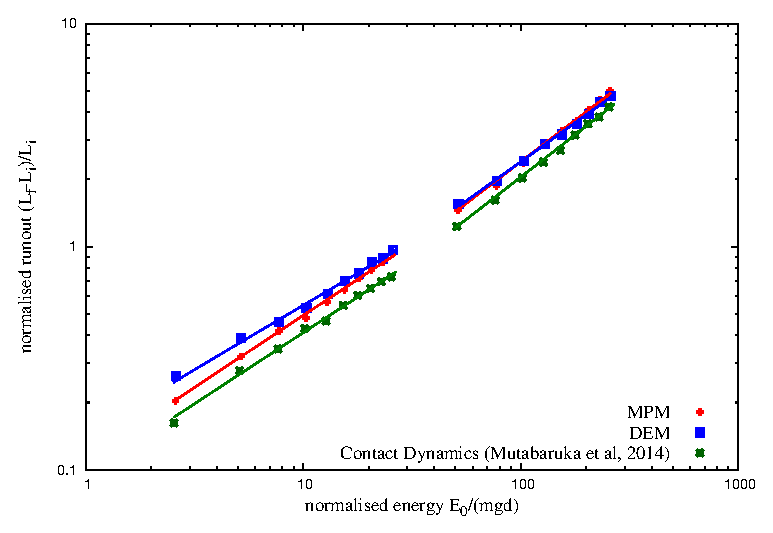
\includegraphics[width=\textwidth]{Runout_Eo_MPM_CD_DEM}
\caption{Run-out distance as a function of normalised input kinetic energy.}
\label{fig:Runout_Eo_MPM_CD_DEM}
\end{subfigure}
\\
\begin{subfigure}[b]{0.975\textwidth}
\centering
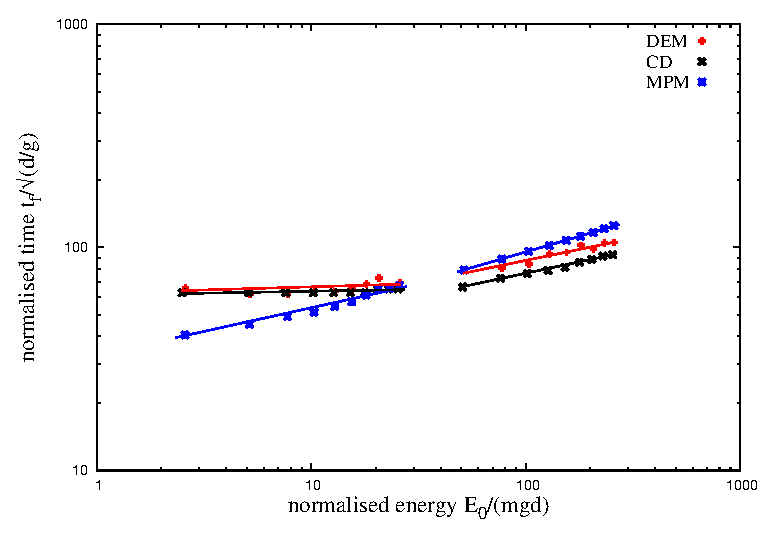
\includegraphics[width=\textwidth]{Tf_vs_Eo_Slope}
\caption{Duration of run-out as a function of normalised input kinetic energy.}
\label{fig:Tf_vs_Eo_Slope}
\end{subfigure}
\caption{Evolution of run-out and time as a function of the normalised input 
energy for a pile subjected a gradient horizontal energy.}
\label{fig:Slope}
\end{figure}

In the second regime, corresponding to the range of high input energies  $E_0 > 
40 \ mgd$, the run-out distance varies as $L_f \propto (E_0)^{\alpha'}$ over 
one decade with $\alpha' \simeq 0.56\pm 0.04$ while the duration increases as 
$t_f \propto (E_0)^{\beta'}$ with $\beta' \simeq 0.33 \pm 0.02$. Hence, in this 
regime the average run-out speed varies as $v_s \propto (E_0)^{0.498 \pm 
0.01}$. This exponent is close to the value $0.5$ in $v_0 \propto (E_0)^{0.5}$, 
and hence, within the confidence interval of the exponents.
%, in the second 
%regime we may assume $\beta' \simeq \alpha' - 0.5$ and $v_s \propto v_0$. 
In the second regime, both DEM and MPM predict almost the same run-out 
behaviour. However, MPM predicts longer duration with increase in the input 
energy.

It is worth noting that a similar power-law dependence of the run-out distance 
and time are found in the case of granular column collapse with respect to 
the initial aspect ratio. In the column geometry, the grains spread away 
owing to the kinetic energy acquired during gravitational collapse of the 
column.~\citet{Topin2012} found that the run-out distance varies as a power-law 
of the available peak kinetic energy at the end of the free-fall stage with an 
exponent $\simeq 0.5$. This value of exponent is lower than the run-out 
evolution observed in the second regime. This is, however, physically plausible 
since the distribution of kinetic energies at the end of the collapse 
is more chaotic than in this case where the energy is supplied from the very 
beginning in a well-defined shear mode. As pointed out by~\citet{Staron2005}, 
the distribution of kinetic energies is an essential factor for the run-out 
distance.

%-------------------------------------------------------------------------------------------
\subsection{Decay of kinetic energy}
\label{sec:decay}

The non-trivial evolution of the pile geometry in two regimes suggests that 
the energy supplied to the pile is not simply dissipated by shear and friction 
along the bottom plane. It is important to split the kinetic energy into 
vertical and horizontal components ($K_{Ex}$ and $K_{Ey}$) of the velocity 
field. Although, the input energy is in the $x$ component, a fraction of 
the energy is transferred to the vertical component of the velocity field and 
dissipated during the transient phase. The evolution of kinetic energy is 
studied to understand the behaviour of granular flow that is consistent with 
the evolution of the pile shape.

The evolution of total kinetic energies $E_k$ with time for different values of 
the input energy $E_{ki}$ based on MPM simulations are shown 
in~\cref{fig:Energy_Time_Slope}. The MPM simulation shows two distinct regimes 
in the normalised kinetic energy plot as a function of normalised time 
in~\cref{fig:Normalised_Energy_Time_Slope}. However, the DEM simulations 
(\cref{fig:Normalised_Energy_Time_Slope_DEM}) show that the energy evolution 
corresponding to the low energy regime nearly collapse on to a single time 
evolution. This is consistent with the observation of run-out time $t_f$ being 
independent of the input energy. In contrast, MPM simulations predict a power 
law relation between the run-out duration and input energy. However, the 
plots corresponding to the high energy regime (\cref{fig:Energy_Time_Slope}), 
collapse only at the beginning of the run-out i.e. for $t < t_1 \simeq 7.5 \ 
(d/g)^{0.5}$. Although MPM simulations show a longer duration of run-out 
(\cref{fig:Energy_Time_Slope}), the total kinetic energy is completely 
dissipated at $t = 60 \sqrt{d/g}$. DEM simulations predict $t = 80 \sqrt{d/g}$ 
for the kinetic energy to be completely dissipated. This is due to grain 
rearrangement at the free surface (\cref{fig:voro_500}). The granular mass 
densifies as the flow progresses, after the initial dilation phase for $t = 
20\sqrt{d/g}$.

\begin{figure}[tbhp]
\centering
\begin{subfigure}[b]{0.975\textwidth}
\includegraphics[width=\textwidth]{Energy_Slope}
\caption{Evolution of total kinetic energy with time.}
\label{fig:energy_slope}
\end{subfigure}
\\
\begin{subfigure}[b]{0.975\textwidth}
\centering
\includegraphics[width=\textwidth]{Normalised_Energy_Time_Slope}
\caption{Evolution of normalised kinetic energy with normalised time.}
\label{fig:Normalised_Energy_Time_Slope}
\end{subfigure}
\caption{Evolution of kinetic energy with time (MPM) for a pile subjected to 
gradient input velocities.}
\label{fig:Energy_Time_Slope}
\end{figure}

\begin{figure}[tbhp]
\centering
\includegraphics[width=0.9\textwidth]{Normalised_Energy_Time_Slope_DEM}
\caption{Evolution of normalised kinetic energy with normalised time for a pile 
subjected to gradient input velocities.}
\label{fig:Normalised_Energy_Time_Slope_DEM}
\end{figure}

\begin{figure}[tbhp]
\centering
\includegraphics[width=0.9\textwidth]{voro_500}
\caption{Evolution of packing density with time $E_0 = 152 mgd$ (DEM).}
\label{fig:voro_500}
\end{figure}

\Cref{fig:Normalised_KEx_KEy_Slope} displays the evolution of kinetic energy 
in the translational ($E_x$ and $E_y$) degrees of freedom. $E_x$ decays similar 
to the total energy dissipation, but $E_y$ increases and passes through a peak 
before decaying rapidly to a negligible level. The transient is best 
observed for $E_y$, which has significant values only for $t< t_1$. This energy 
represents the proportion of kinetic energy transferred to the $y$ component of 
the velocity field  due to the destabilisation of the pile and collapse of 
grains in the cavity behind the pile. Higher proportion of vertical 
acceleration $E_{ky}/E_0$ is observed for lower values of input energy $E_0$. 
This means that, at lower input energies a larger fraction of the energy is 
consumed in the destabilisation process. Whereas at a higher input energies, 
most of the energy is dissipated in the spreading phase. For this reason, the 
total duration $t_1$ of this destabilisation phase is nearly the same in 
both regimes and its value is controlled by gravity rather than the input 
energy. The height of the pile being of the order of $80 \ d$, the total 
free-fall time for a particle located at this height is $\simeq 12 \ 
(d/g)^{0.5}$, which is of the same order as $t_1$. DEM simulations show that 
the contribution of the rotational energy during the transient stage and the 
spreading stage is negligible. 

\begin{figure}[tbhp]
\centering
\begin{subfigure}[b]{0.975\textwidth}
\includegraphics[width=\textwidth]{Normalised_KEx_Slope}
\caption{Evolution of normalised horizontal kinetic energy with time.}
\label{fig:Normalised_KEx_Slope}
\end{subfigure}
\\
\begin{subfigure}[b]{0.975\textwidth}
\centering
\includegraphics[width=\textwidth]{Normalised_KEy_Slope}
\caption{Evolution of normalised vertical kinetic energy with time.}
\label{fig:Normalised_KEy_Slope}
\end{subfigure}
\caption{Evolution of vertical and horizontal kinetic energy with time (MPM) 
for a pile subjected to gradient input velocities.}
\label{fig:Normalised_KEx_KEy_Slope}
\end{figure}

To analyse the second phase for higher input energies, the 
kinetic energy $E'_{kx0}$ at the end of the transient phase is 
considered. This energy is responsible for most of the run-out, hence it is 
expected to 
control the run-out distance and time.~\Cref{fig:Normalised_KExExop_Slope} 
shows the evolution of $E_{kx}$ normalised by $E'_{kx0}$ as a function of time. 
The plots have seemingly the same aspect but they show different decay times. A 
decay time $\tau$ can be defined as the time required for $E_{kx}$ to decline 
by a factor $1/2$.~\Cref{fig:ExEx0_vs_ttau} shows the same data in 
which the time $t'$ elapsed since $t_1$, normalised by $\tau$. Interestingly, 
now all the data nicely collapse on to a single curve. However, this curve can 
not be fitted by simple functional forms such as variants of exponential decay. 
This means that the spreading of the pile is not a self-similar process in 
agreement with the fact that the energy fades away in a finite time $t'_f$. 

\clearpage

\begin{figure}[tbhp]
\centering
\includegraphics[width=\textwidth]{Normalised_KExExop_Slope}
\caption[Evolution of the normalised horizontal kinetic energy as function of 
time since the transient phase.]{Evolution of kinetic energy in the $x$ 
component of the velocity field normalised by the available kinetic energy at 
the
end of the transient phase as a function of time elapsed since the
same instant (MPM).}
\label{fig:Normalised_KExExop_Slope}
\end{figure}

\begin{figure}[tbhp]
\centering
\includegraphics[width=\textwidth]{EkxKoTTau_Slope}
\caption[Evolution of the normalised horizontal kinetic energy as function of 
the normalised time since the transient phase.]{Evolution of kinetic energy in 
the $x$ component of 
the velocity field  normalised by the available kinetic energy at the end of 
the transient as a function of normalised time (MPM).}
\label{fig:ExEx0_vs_ttau}
\end{figure}


The scaling of the data with the decay time $\tau$ suggests that the 
run-out time, since the beginning of the second phase, $t'_f$ might be a simple 
function of $\tau$.~\Cref{fig:tp_tau_mgd} shows both $t'_f$ and $\tau$ as 
a function of $E'_{x0}$, where a power-law relation can be observed for both 
time scales. The run-out time $t'_f \propto (E'_{x0})^{\beta'}$ has the 
same exponent $\beta' \simeq 0.33 \pm 0.02$ as $t_f$ as a function of $E_0$. 
For the decay time we have $\tau \propto (E'_{x0})^{\beta''}$ with $\beta'' 
\simeq 0.38 \pm 0.03$. The relation between the two times can thus be expressed 
as (\cref{fig:tpTau})
\begin{equation}
t'_f = k  \ \tau \, (E'_{x0})^{\beta'' - \beta'} \,,
\label{eqn:t'f}
\end{equation}
where $k \simeq 5.0 \pm 0.4$ and $\beta'' - \beta' \simeq 0.05 \pm 0.05$. This 
value is small enough to be neglected. It is therefore plausible to assume that 
the run-out time is a multiple of the decay time and the spreading process is 
controlled by a single time. A weak dependence on the energy $E'_{kx0}$ is 
consistent with the fact that the energy available at the beginning of the 
second phase is not dissipated in the spreading process (calculated from the 
position of the tip of the pile) since the pile keeps deforming by the 
movements of the grains at the free surface even when the tip comes to rest. 
This can explain the small difference between the two exponents as observed 
here.


\begin{figure}[tbhp]
\centering
\begin{subfigure}[b]{0.975\textwidth}
\includegraphics[width=\textwidth]{tp_tau_mgd}
\caption{Power law evolution of $t'_f$ and $\tau$ as a function of kinetic 
energy $E'_{kx0}$.}
\label{fig:tp_tau_mgd}
\end{subfigure}
\\
\begin{subfigure}[b]{0.975\textwidth}
\centering
\includegraphics[width=\textwidth]{tpTau}
\caption{Linear relationship between decay time and run-out time after the 
transient as a function of the normalised kinetic energy $E_{kx0}$.}
\label{fig:tpTau}
\end{subfigure}
\caption{Decay time and run-out time as a function of the normalised kinetic 
energy $E_{kx0}$.}
\label{fig:tp_Tau}
\end{figure}


%-------------------------------------------------------------------------------
\subsection{Effect of friction}
\label{sec:parameters}

The run-out distance, duration of flow, and the dissipation of kinetic energy 
are controlled by the input energy and collective dynamics of the whole pile. 
However, the run-out behaviour is also expected to depend on the base friction. 
A series of simulations with different values of base friction was performed 
using MPM to analyse the influence of friction on the run-out behaviour. The 
influence of friction on the run-out behaviour for different input energies is 
shown in~\cref{fig:runout_fric_slope}. The run-out distance decreases with 
increase in the basal friction. The exponent of the 
power-law relation between the run-out and input energy has a weak dependence 
on the base friction, however, the proportionality constant is affected by the 
change in the base friction. This behaviour is similar to that observed in 
granular column collapse with varying initial 
properties~\citep{Balmforth2005,Lajeunesse2005}. 

CD simulations using different values of coefficient of restitution show no 
difference in the run-out behaviour. At large input energies, the pile remains 
in a dense state so that multiple collisions inside the pile occur at small 
time scales compared to the deformation time. When the restitution coefficients 
are increased, more collisions occur during a longer time interval but the 
overall energy dissipation rate by collisions remains the same. This effect is 
a seminal example of collective effects which erase the influence of local 
parameters at the macroscopic scale.

In contrast to the restitution coefficients, the effect of friction 
coefficient is quite important for the run-out. MPM simulations with 
varying friction coefficient show that, both the run-out distance and the 
decay time decrease as the friction coefficient is increased. This 
effect is much more pronounced at low values of the friction coefficient. 
The run-out time, for example, is reduced by a factor of approximately 4 as 
$\mu_s$ is increased from 0.1 to 0.2 while the change in the run-out and 
duration is less affected with increase in friction coefficient. This 
``saturation effect'' can be observed in a systematic way in simple shear 
tests. The dissipation rate may reach a saturation point where the dilation of 
granular materials and rolling of the grains change in response to increase in 
friction coefficient~\citep{Estrada2008}.

\begin{figure}[tbhp]
\centering
\begin{subfigure}[b]{0.95\textwidth}
\centering
\includegraphics[width=\textwidth]{runout_fric_slope}
\caption{Effect of friction on the run-out distance}
\label{fig:runout_fric_slope}
\end{subfigure}
\\
\begin{subfigure}[b]{0.95\textwidth}
\centering
\includegraphics[width=\textwidth]{time_fric_slope}
\caption{Effect of friction on the duration of run-out.}
\label{fig:time_fric_slope}
\end{subfigure}
\caption{MPM simulations of effect of friction on the run-out behaviour of 
slopes subjected to horizontal excitation.}
\label{fig:fric_slope}
\end{figure}

%-------------------------------------------------------------------------------

\subsection*{Effect kinetic energy distribution}

\citet{Staron2005} observed that the distribution of kinetic energy in the 
granular system is an essential factor for the run-out distance. In order to 
understand the influence of energy distribution on the run-out behaviour, 
granular pile subjected to two different velocity fields are studied. A 
uniform velocity $V_{xo} (y) = V_0$ is applied to the entire pile, in contrast 
to the gradient horizontal velocity. Snapshots of flow kinematics at initial 
stages are shown in~\cref{fig:Uniform_Slope_Profile_200J} (MPM simulations) 
and~\cref{fig:Uniform_Slope_DEM_200J} (DEM). It can be observed from the 
figures that the continuum behaviour is identical to that of grain-scale 
simulations. As each grain experiences the same velocity, grains located at the 
top of the slope are pushed farther away and unlike the gradient input 
velocity, the cavity left behind the granular mass is not filled by the soil 
grains at the top. 

\Cref{fig:Runout_Eo_GU} shows the influence of velocity distribution on the 
run-out behaviour. At low input energy, the gradient velocity distribution 
shows significantly longer run-out in comparison to uniform velocity 
distribution.~\Cref{sec:decay} shows that at low input energies a larger 
fraction of the energy is consumed in the destabilisation process. This means 
that the amount energy available for flow is less in uniform velocity 
distribution than the gradient velocity profile, this energy is even smaller as 
the initial velocity is distributed uniformly throughout the granular mass. 
However at higher input energy, where most of the energy is dissipated during 
the spreading phase, the run-out distance has a weak dependence on the 
distribution of velocity in the granular mass. The duration of the flow shows 
similar behaviour to the run-out, however, a slope subjected to a gradient 
velocity flows quicker than a slope subjected to a uniform horizontal velocity. 
The gradient velocity distribution provides more input energy at the initial 
stage to overcome the frictional resistance at the base. This shows that the 
material property and the distribution of kinetic energy in the system has a 
non-trivial influence on the flow kinematics and the internal flow structure.



\begin{figure}[tbph]
\centering
\includegraphics[width=\textwidth]{Uniform_Slope_Profile_200J}
\caption{Snapshots of MPM simulations of the evolution of granular pile 
subjected to a gradient horizontal energy $E_0 = 61 \ mgd$.}
\label{fig:Uniform_Slope_Profile_200J}
\end{figure}

\begin{figure}[tbph]
\centering
\includegraphics[width=\textwidth]{Uniform_Slope_DEM_200J}
\caption{Snapshots of DEM simulations of the evolution of granular pile 
subjected to a gradient horizontal energy $E_0 = 61 \ mgd$.}
\label{fig:Uniform_Slope_DEM_200J}
\end{figure}

\begin{figure}[tbph]
\centering
\begin{subfigure}[b]{0.95\textwidth}
\centering
\includegraphics[width=\textwidth]{Runout_Eo_GU}
\caption{Run-out distance as a function of normalised input kinetic energy.}
\label{fig:Runout_Eo_GU}
\end{subfigure}
\\
\begin{subfigure}[b]{0.95\textwidth}
\centering
\includegraphics[width=\textwidth]{time_Eo_GU}
\caption{Duration of run-out as a function of normalised input kinetic energy.}
\label{fig:time_Eo_GU}
\end{subfigure}
\caption{Effect of input velocity distribution on the run-out behaviour of 
slopes subjected to horizontal velocities.}
\label{fig:GU}
\end{figure}
%-------------------------------------------------------------------------------

\subsection{Comparison with granular column collapse}

\Cref{fig:Runout_Slope_Column} shows the run-out behaviour of granular column 
collapse and the slope subjected to horizontal excitations as a function of 
normalised kinetic energy. In the case of column collapse, the peak energy at 
$\tau_c$ is used as the energy available for the flow. It can be observed that 
MPM and DEM predict similar run-out behaviour for low energy regime (short 
columns), which undergo frictional failure along the flanks. However MPM 
predicts longer run-out for high energy regime (corresponding to a > 2.7), 
where the granular column experiences significant collisional dissipation. The 
lack of a collisional energy dissipation mechanism in MPM results in over 
prediction of run-out distances. In the case of granular column subjected to 
horizontal velocity, the dissipation is friction and MPM is able to predict the 
run-out response in good agreement with DEM simulations. At very low energy, 
DEM simulations show longer run-out in the case of slope subjected to 
excitations due to local destabilisation at the flow front. Both granular 
flows, column collapse and slope subjected to horizontal excitation, show 
power-law relation with the 
energy. This shows that the power-law behaviour is a granular flow 
characteristic.

\begin{figure}[tbhp]
\centering
\includegraphics[width=0.95\textwidth]{Runout_Slope_Column}
\caption{Comparison of the normalised run-out between the collapse of granular 
columns and granular slope subjected to horizontal loading.}
\label{fig:Runout_Slope_Column}
\end{figure}

%\clearpage

\section{Summary}

Multi-scale simulations of dry granular flows were performed to capture the 
local rheology, and to understand the capability and limitations of continuum 
models in realistic simulation of granular flow dynamics. Previous studies on 
granular collapse have shown a power-law dependence between the run-out and the 
initial aspect ratio of the column. The change in the run-out behaviour for 
tall columns has remained unexplained. Continuum approach predict longer 
run-out distance, however, the reason for this behaviour was still lacking. 
Most studies were focused on mono-disperse grain sizes. In the present study, 
multi-scale simulations of granular column collapse are performed. Studies on 
the role of initial packing density and a poly-disperse sample on the run-out 
behaviour are also performed. The following conclusions can be derived based on 
MPM and DEM simulations of granular column collapse:

\begin{itemize}

\item Both DEM and MPM simulations show a power-law dependence of the run-out 
and time with the initial aspect ratio of the column. 

\item A continuum approach, such as MPM, with a simple frictional dissipation 
model is able to capture the flow kinematics of dry granular collapse for short 
columns. The collapse of a short column is a frictional dissipation process.

\item DEM simulations reveal collisional dissipation mechanism in the initial 
stage of collapse of tall columns. 

\item MPM simulations show longer run-out behaviour in the case 
of tall columns. MPM simulation assumes that the total initial potential energy 
stored in the system is completely dissipated through friction over the entire 
run-out distance. The lack of collisional dissipation in MPM results in longer 
run-outs for tall columns.

\item  The initial configuration and the material properties have a significant 
influence on the run-out behaviour. The run-out distance increases with 
increase in density of granular packing. This effect is significant in the case 
of tall columns. 

\item DEM simulations with different initial packing shows evolution of packing 
density with time.  Hence it is important to consider macroscopic parameters 
like packing fraction and dilatancy behaviour, which are due to meso-scale 
grain arrangements, when modelling the granular system as a continuum.
\end{itemize}

Natural granular flows are triggered by different mechanisms. The distribution 
of kinetic energy in the granular mass is found to have an effect on the flow 
kinematics. A multi-scale analyses of a granular slope subjected to horizontal 
velocities are performed and the following conclusions are derived:

\begin{itemize}

\item A power-law dependence of the run-out distance and time as a 
function of the input energy is observed. The power-law behaviour is found to 
be a generic feature of granular flow dynamics. 

\item The values of the power-law exponents are not simple functions of the 
geometry. 

\item Two regimes with different values of the exponents: 
a low-energy regime and a high-energy regime are observed. 

\item The low energy regime reflects mainly the destabilisation of the pile, 
with a run-out time independent of the input energy.

\item The second regime is governed by the spreading dynamics 
induced by higher input energy. The evolution of granular slope in the 
high-energy regime can be described by a characteristic decay time, which is 
the time required for the input energy to decay by a factor of 0.5.

\item The run-out distance and the decay time decrease as the friction 
increases. This effect is much more pronounced at low values of friction.

\item  At low input energy, the distribution of kinetic energy in the system is 
found have a significant effect on the run-out, as the energy is mostly 
consumed in the destabilisation process. 
 
\item At higher input energy, where most of the energy is dissipated during 
the spreading phase, the run-out distance has a weak dependence on the 
distribution of velocity in the granular mass. 

\item The duration of the flow shows similar behaviour to the run-out, however, 
a slope subjected to a gradient velocity flows quicker than a slope subjected 
to a uniform horizontal velocity. 

\item The material property and the distribution of kinetic energy in the 
system has a non-trivial influence on the flow kinematics and the internal flow 
structure.

\item MPM is successfully able to simulate the transient evolution with a 
single input parameter, the macroscopic friction angle.

\end{itemize}

This study exemplifies the ability of MPM, a continuum approach,  in modelling 
complex granular flow dynamics and opens the possibility of realistic 
simulation of geological-scale flows on complex topographies.
